%!TEX root = ../StrinJet.tex

\section{Simulate with PYTHIA 8 sQCD with CR1 and rope}%
\label{sec:CRorRope}

\begin{figure}[t]
        \begin{center}
                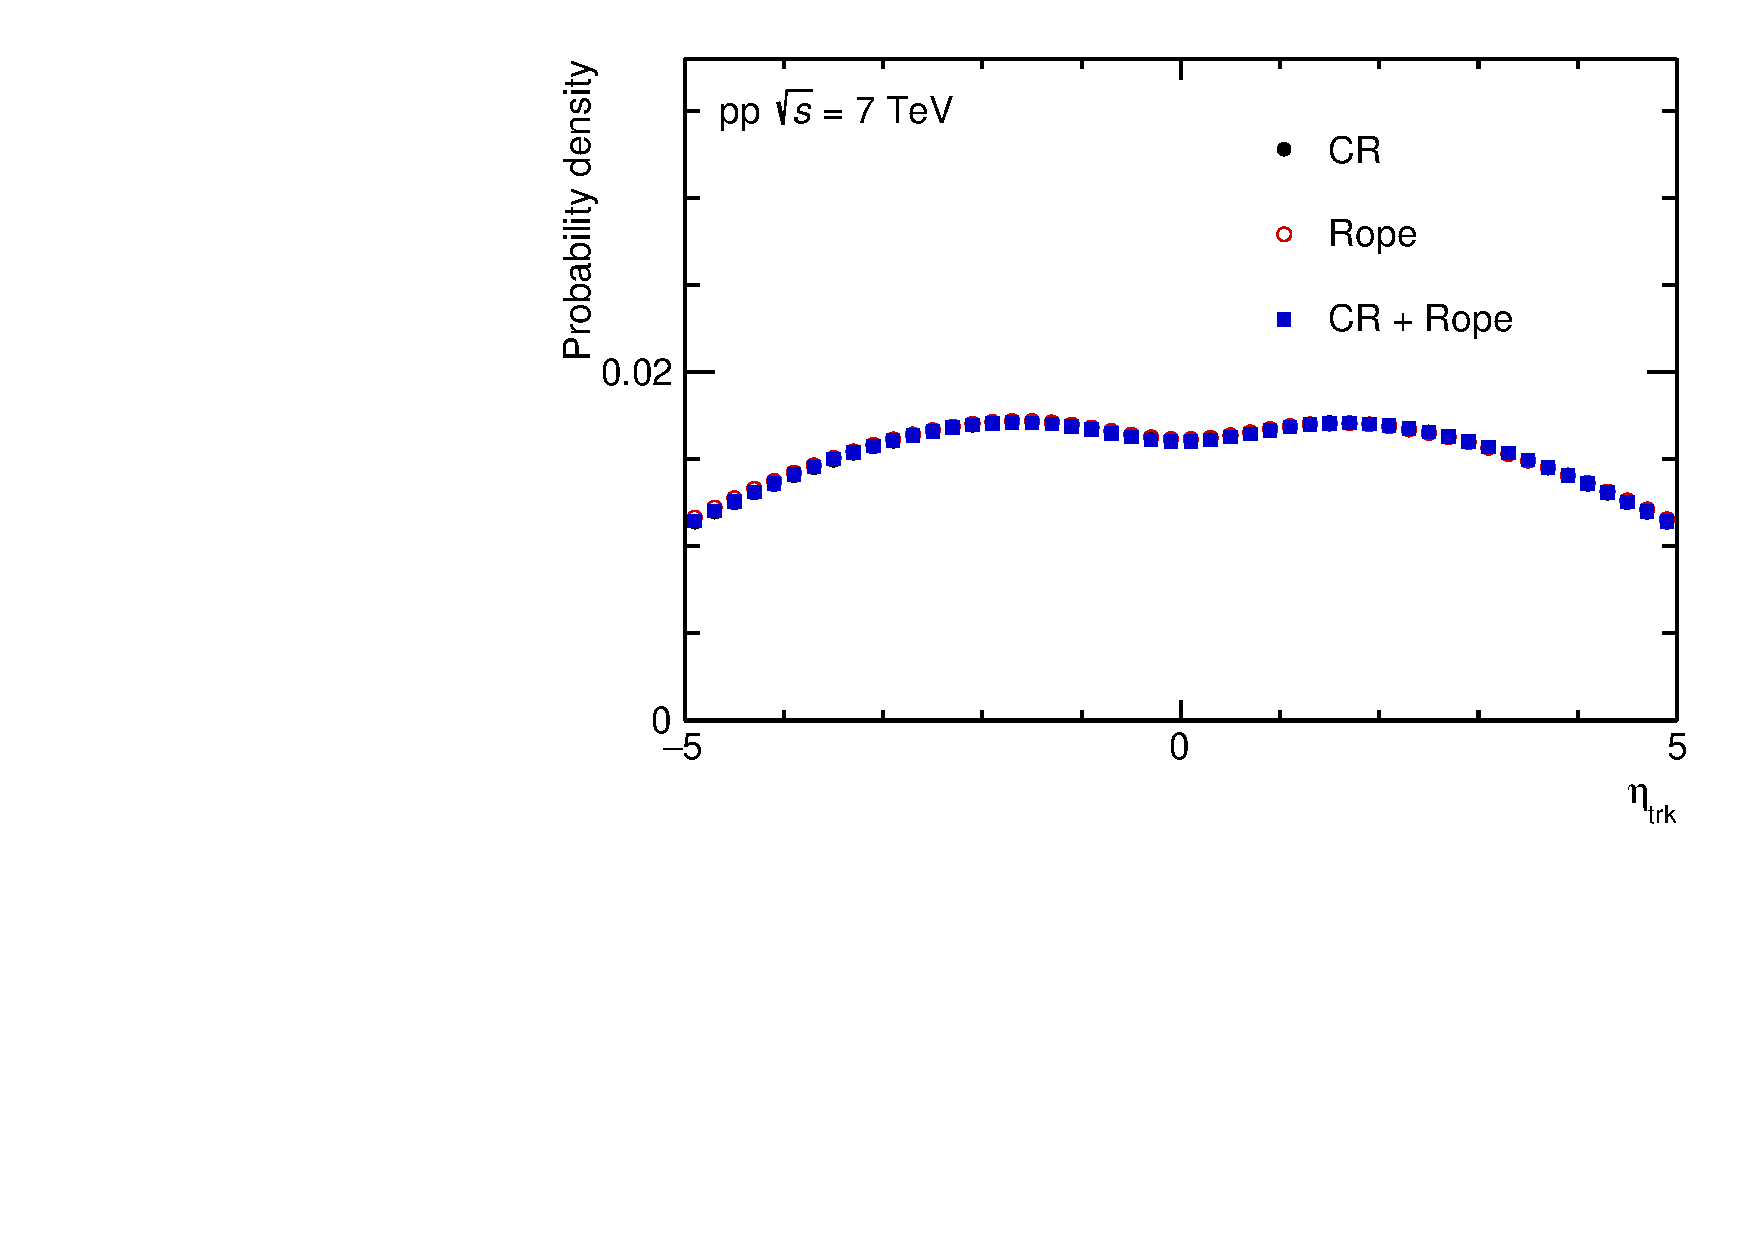
\includegraphics[width=.6\textwidth]{TrkEta}
        \end{center}
        \caption{Track $\eta$ distribution.}
        \label{fig:TrkEta}
\end{figure}

\begin{figure}[t]
	\begin{center}
		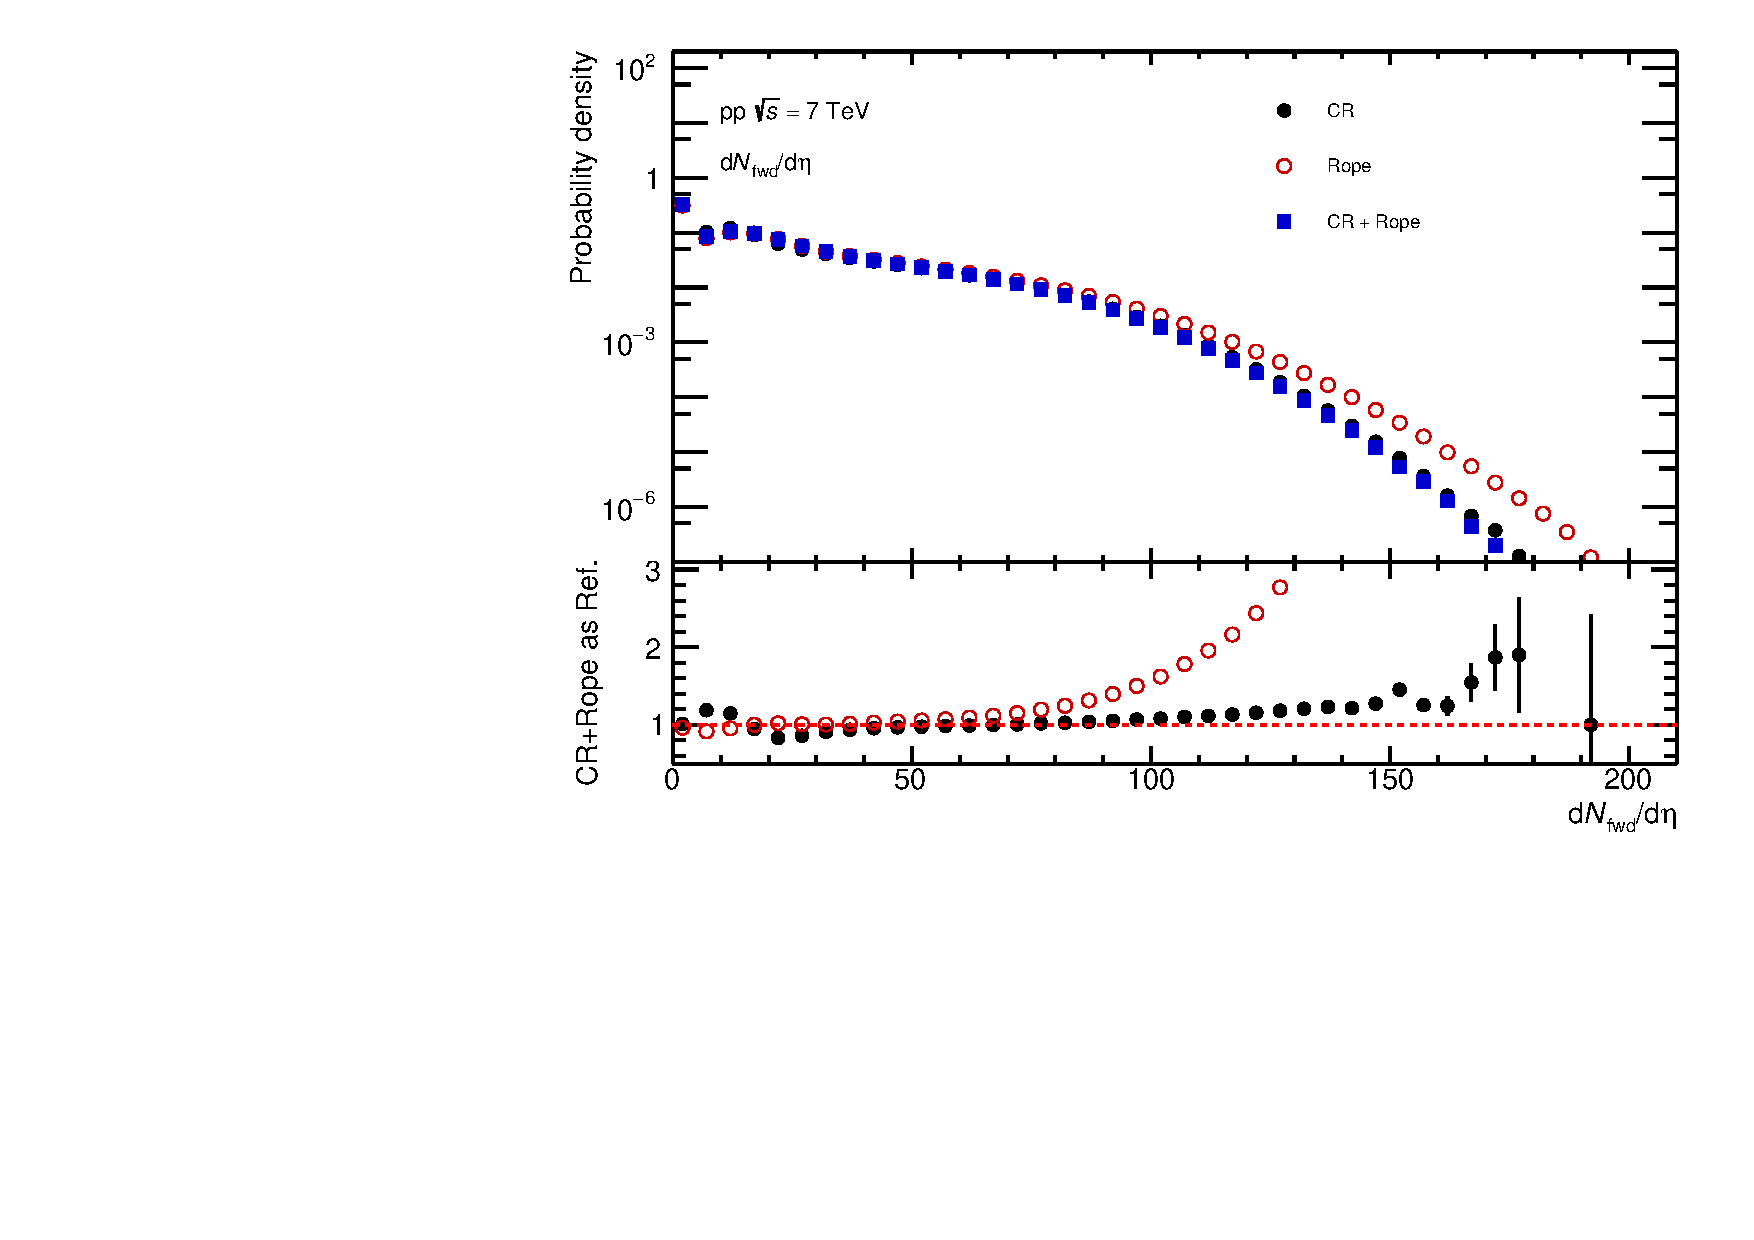
\includegraphics[width=.6\textwidth]{dNfwddEta}
	\end{center}
	\caption{Forward track $\mathrm{d}N_\mathrm{fwd}/\mathrm{d}\eta$ distribution.}
	\label{fig:TrkdNdEta}
\end{figure}

\begin{figure}[ht]
	\begin{center}
		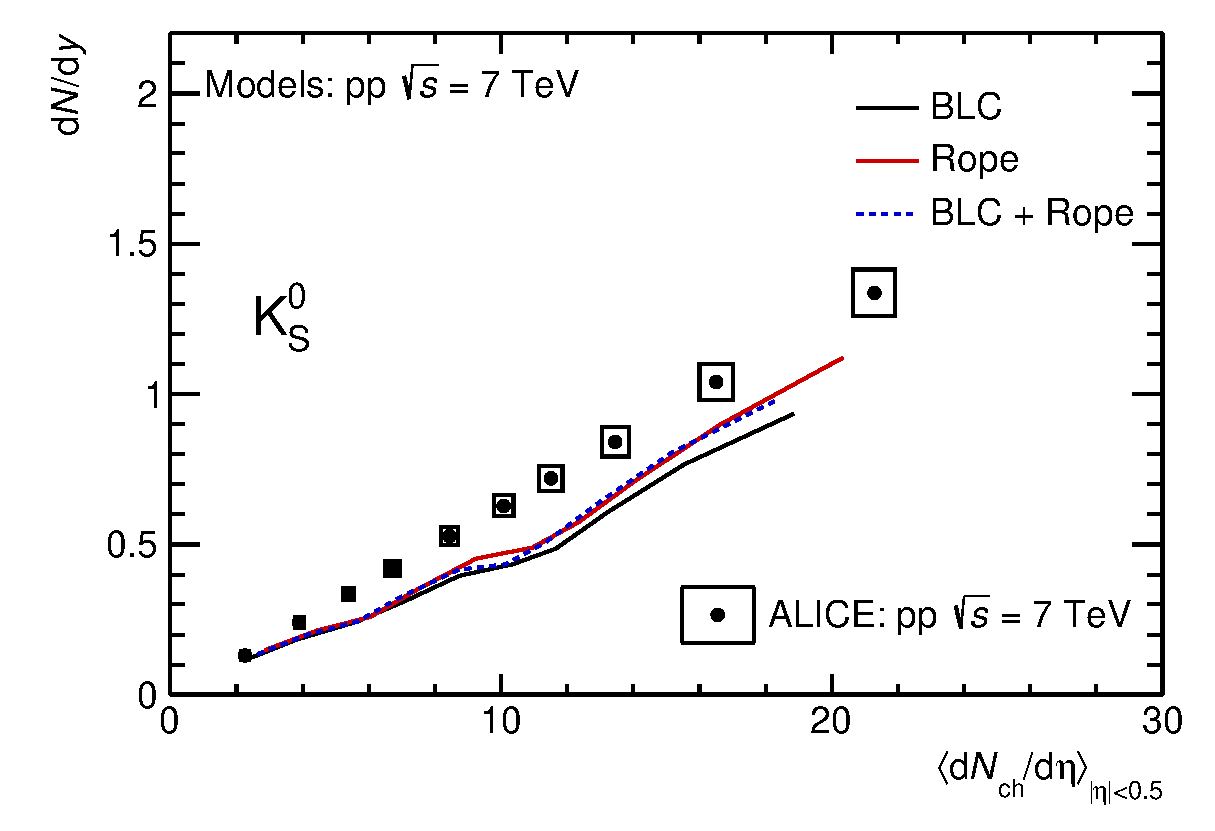
\includegraphics[width=.48\textwidth]{Kshort_InteSpectrum}
		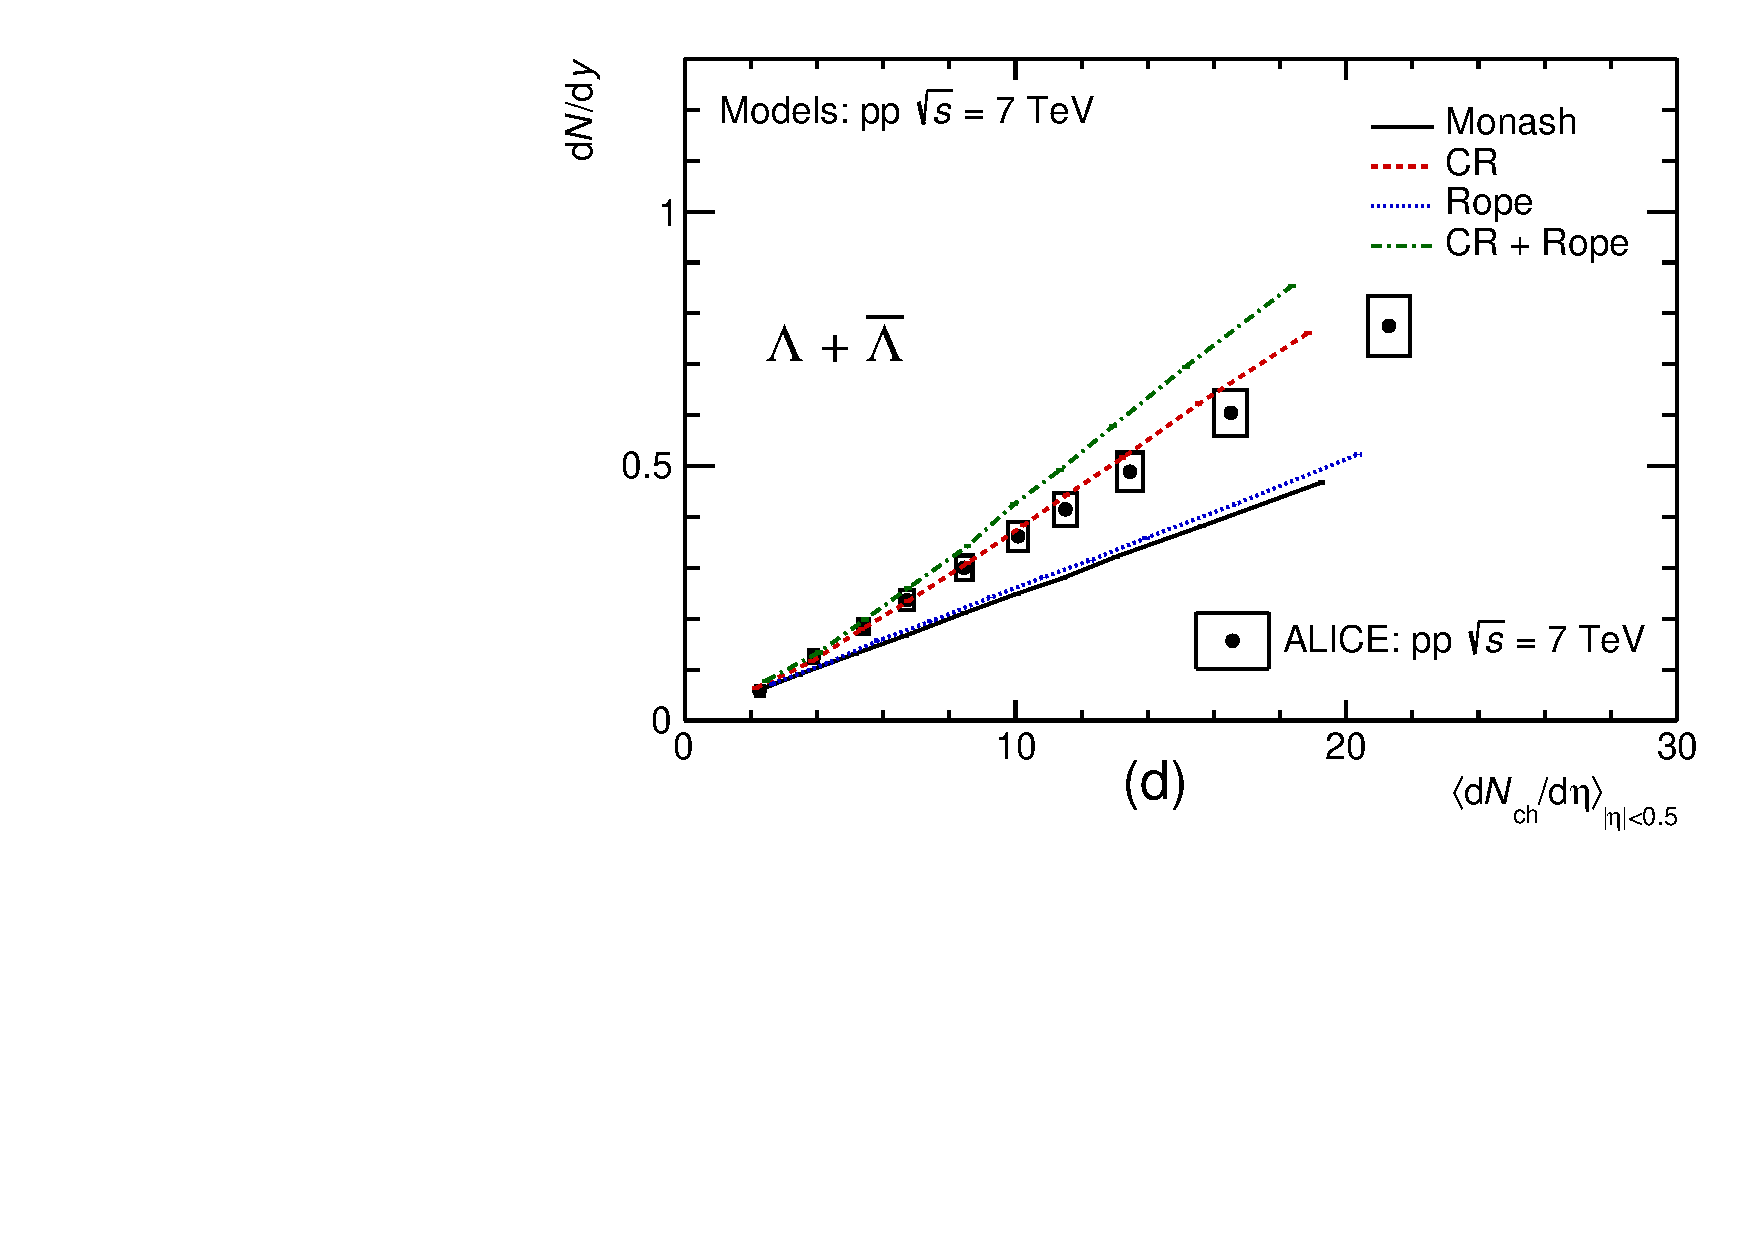
\includegraphics[width=.48\textwidth]{Lambda_InteSpectrum}
		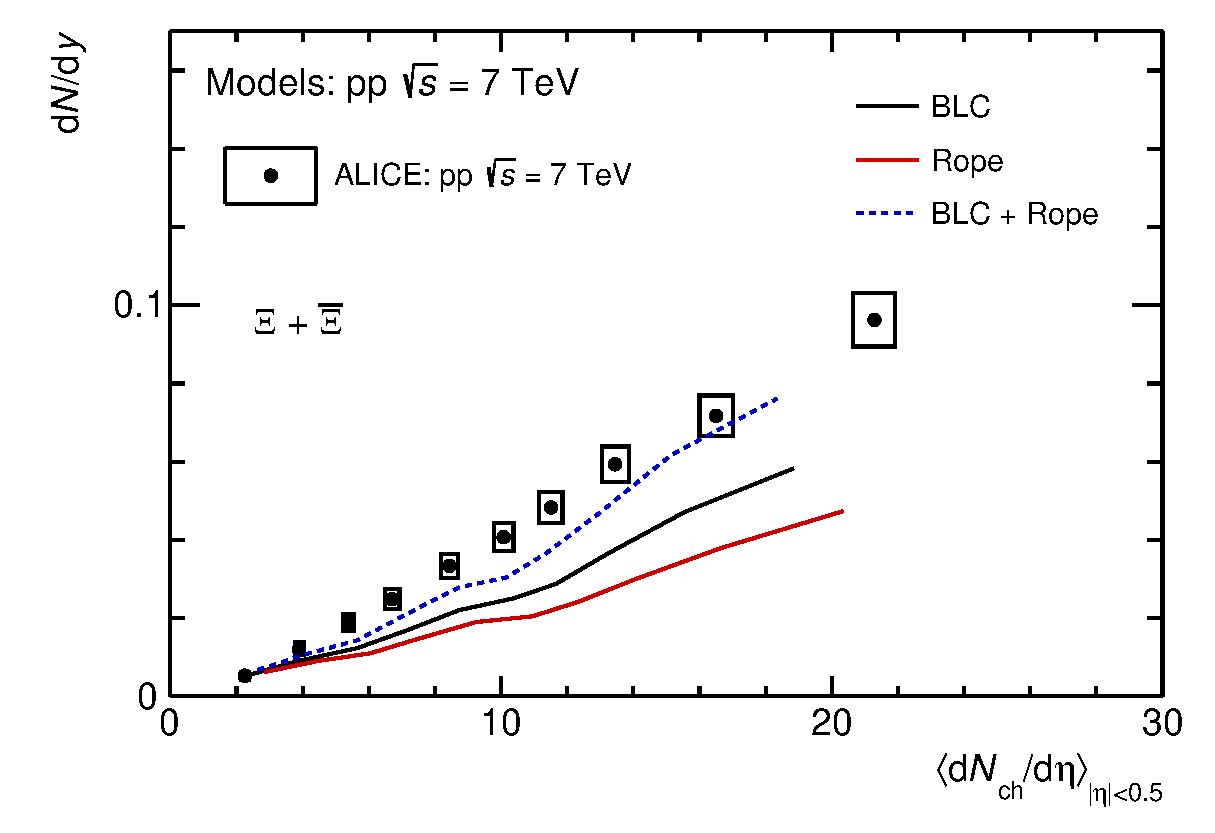
\includegraphics[width=.48\textwidth]{Xi_InteSpectrum}
		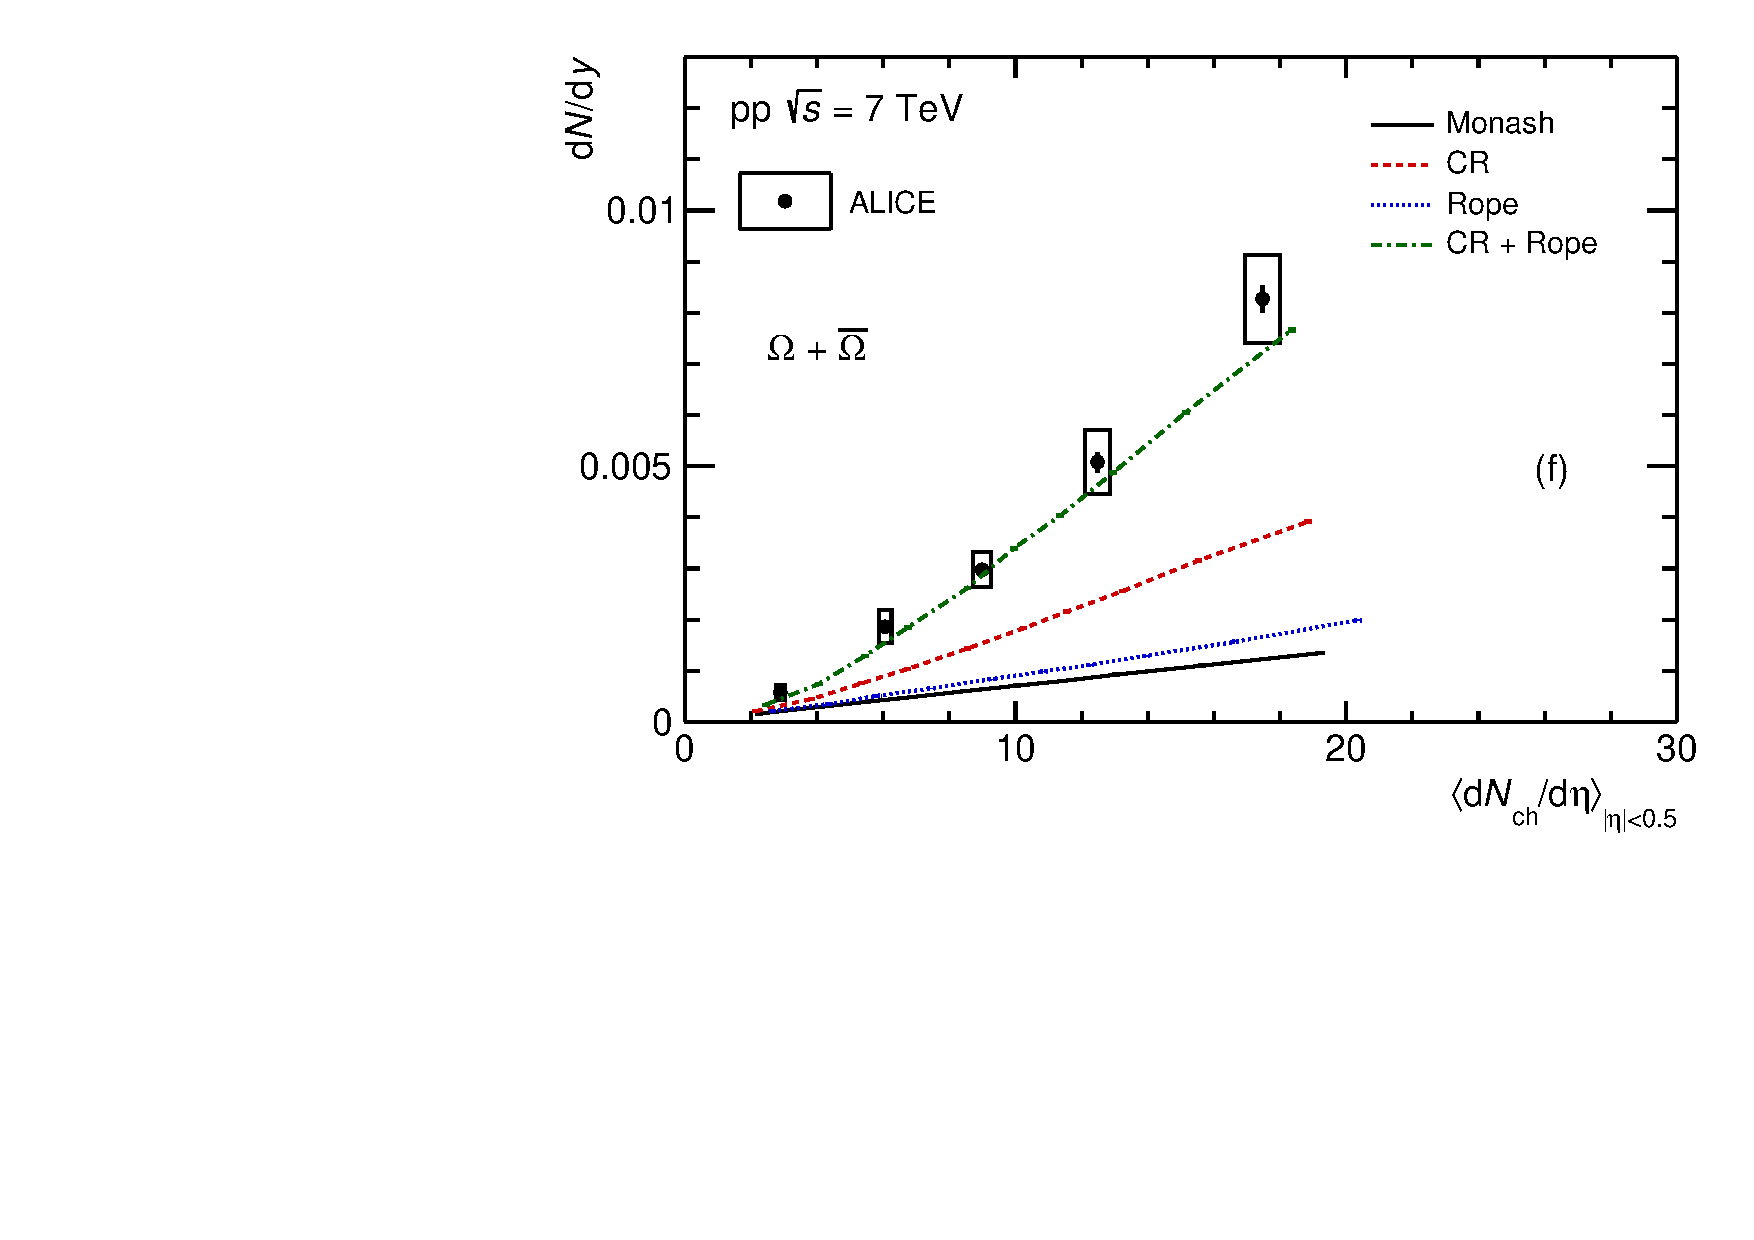
\includegraphics[width=.48\textwidth]{Omega_InteSpectrum}
		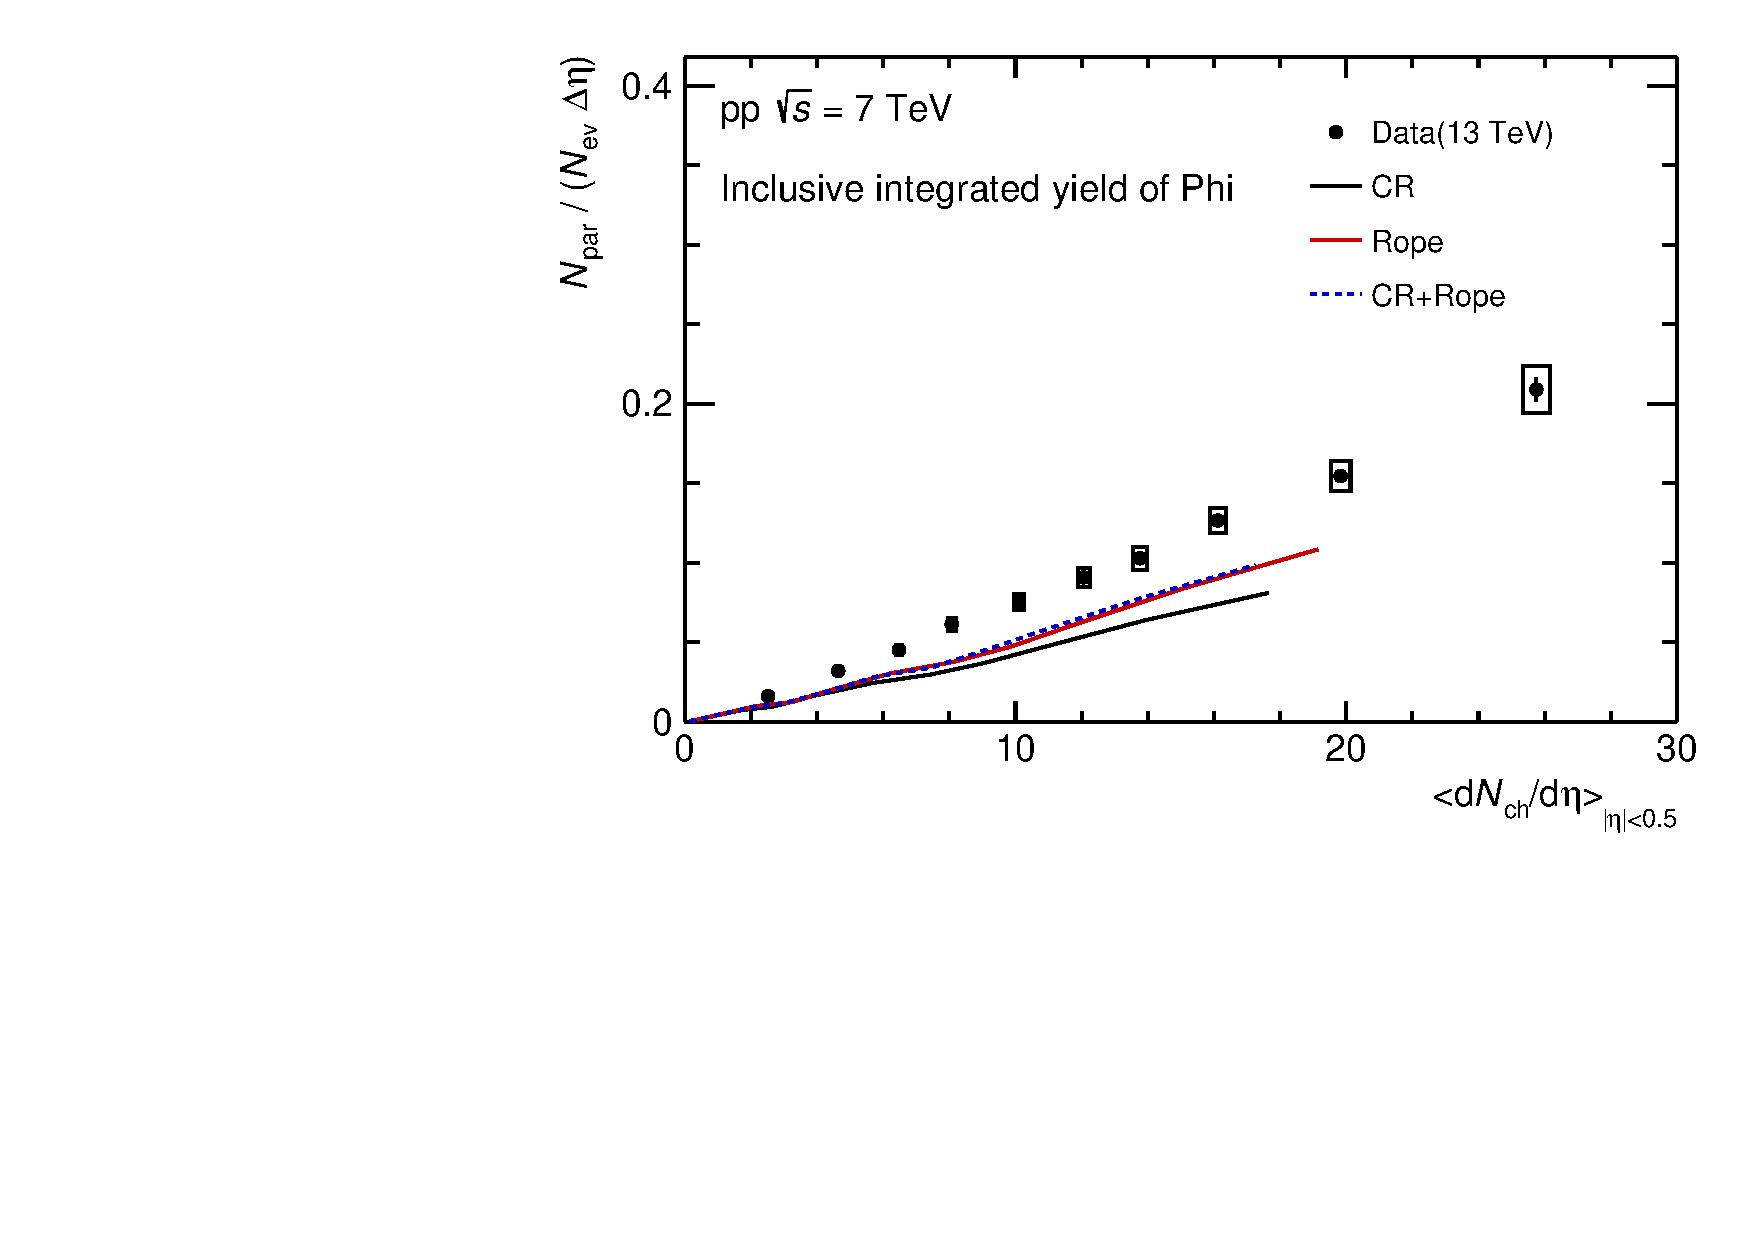
\includegraphics[width=.48\textwidth]{Phi_InteSpectrum}
		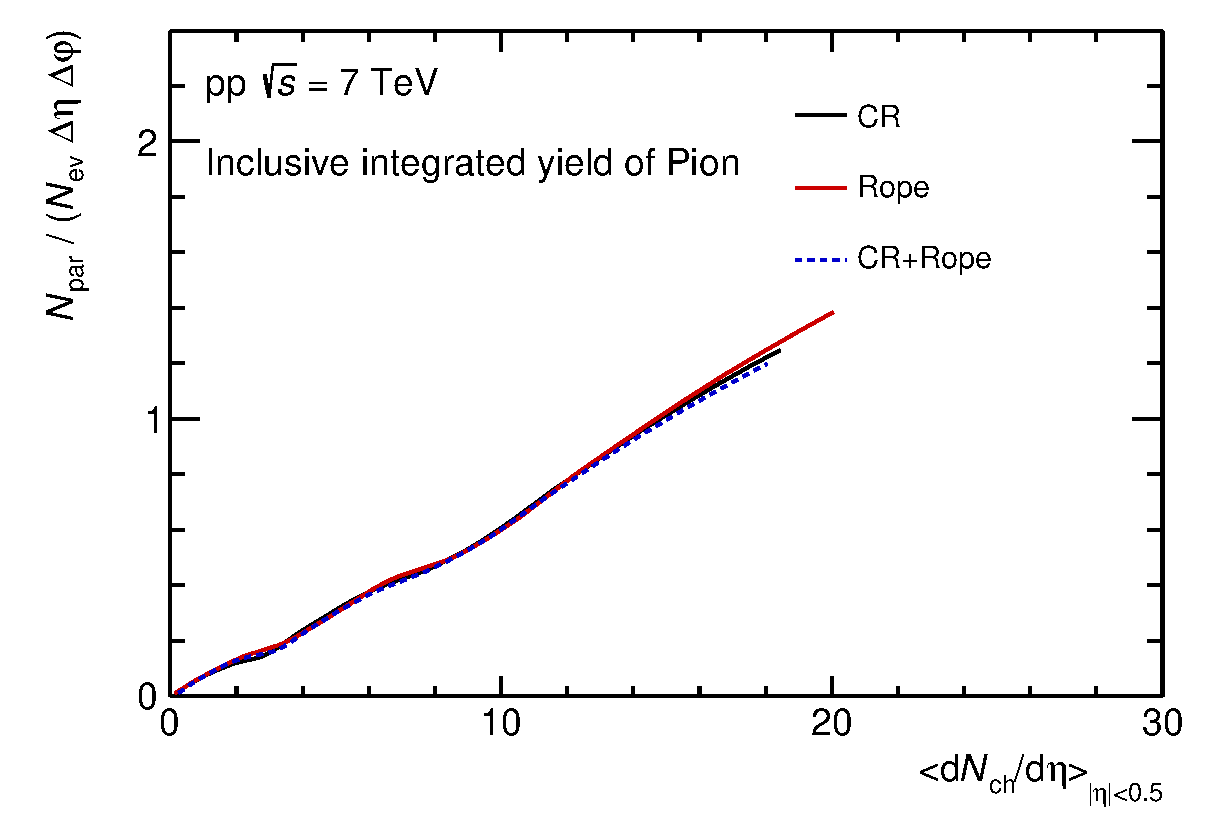
\includegraphics[width=.48\textwidth]{Pion_InteSpectrum}
		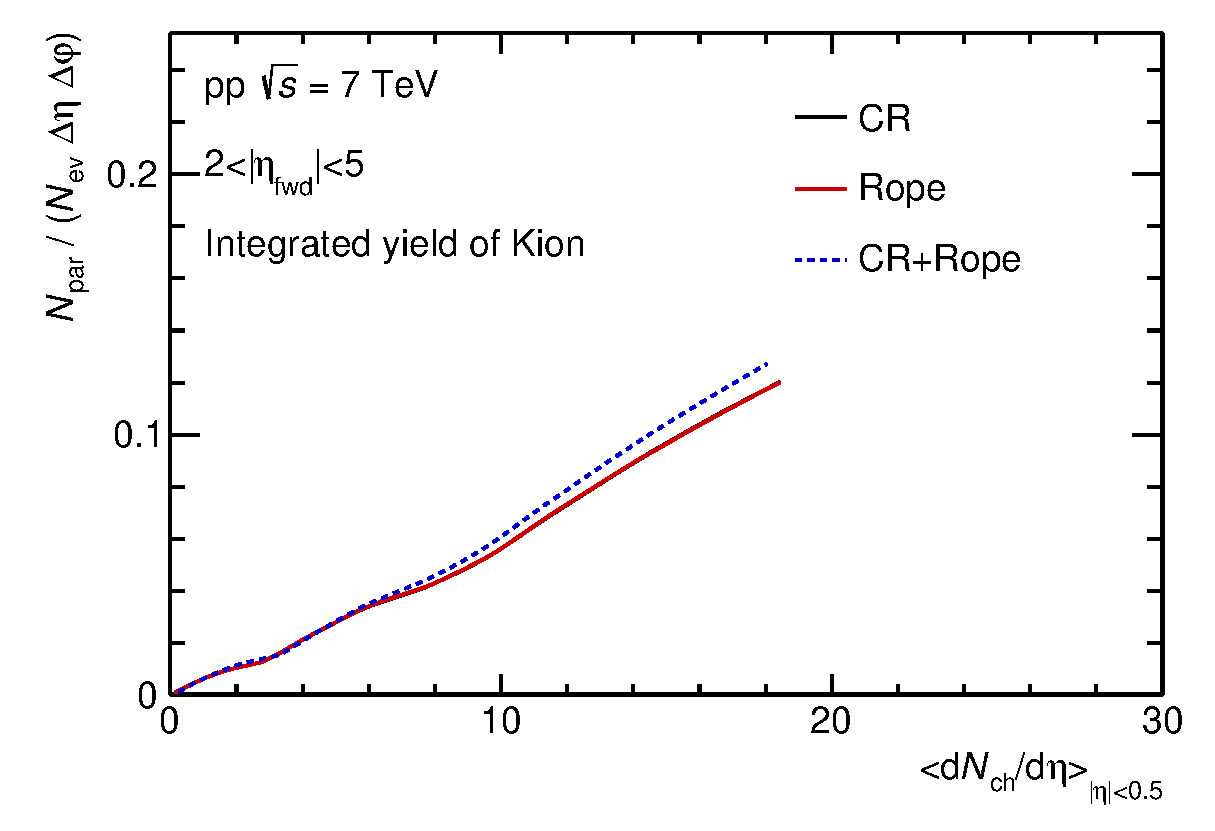
\includegraphics[width=.48\textwidth]{Kion_InteSpectrum}
		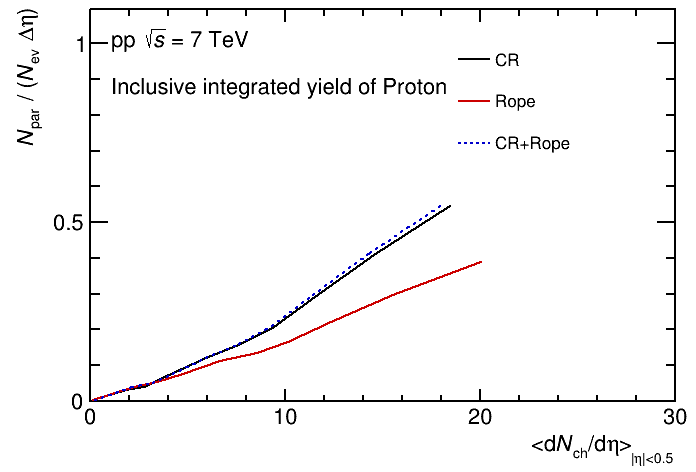
\includegraphics[width=.48\textwidth]{Proton_InteSpectrum}
	\end{center}
	\caption{Inclusive integrated yields of particles with $\avdndeta$.}
	\label{fig:InclIntePar}
\end{figure}

\begin{figure}[ht]
	\begin{center}
		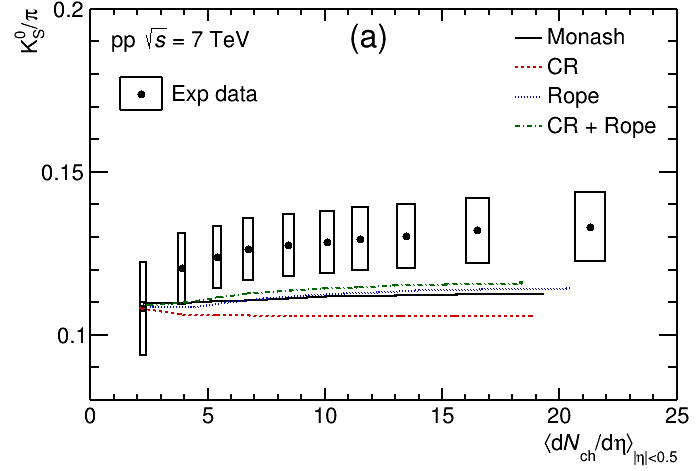
\includegraphics[width=.48\textwidth]{Kshort_PiRatio}
		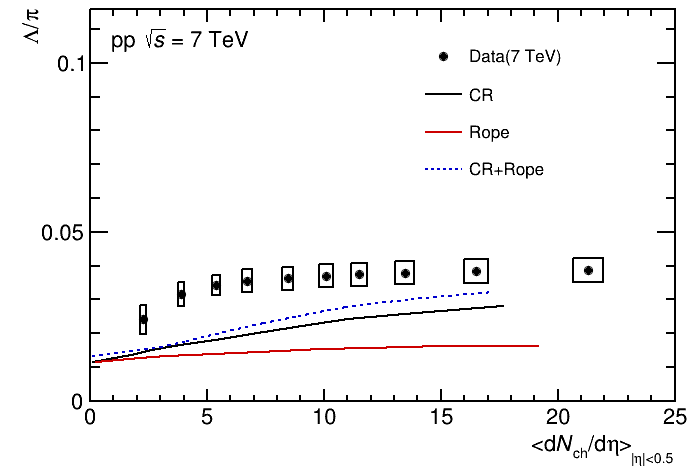
\includegraphics[width=.48\textwidth]{Lambda_PiRatio}
		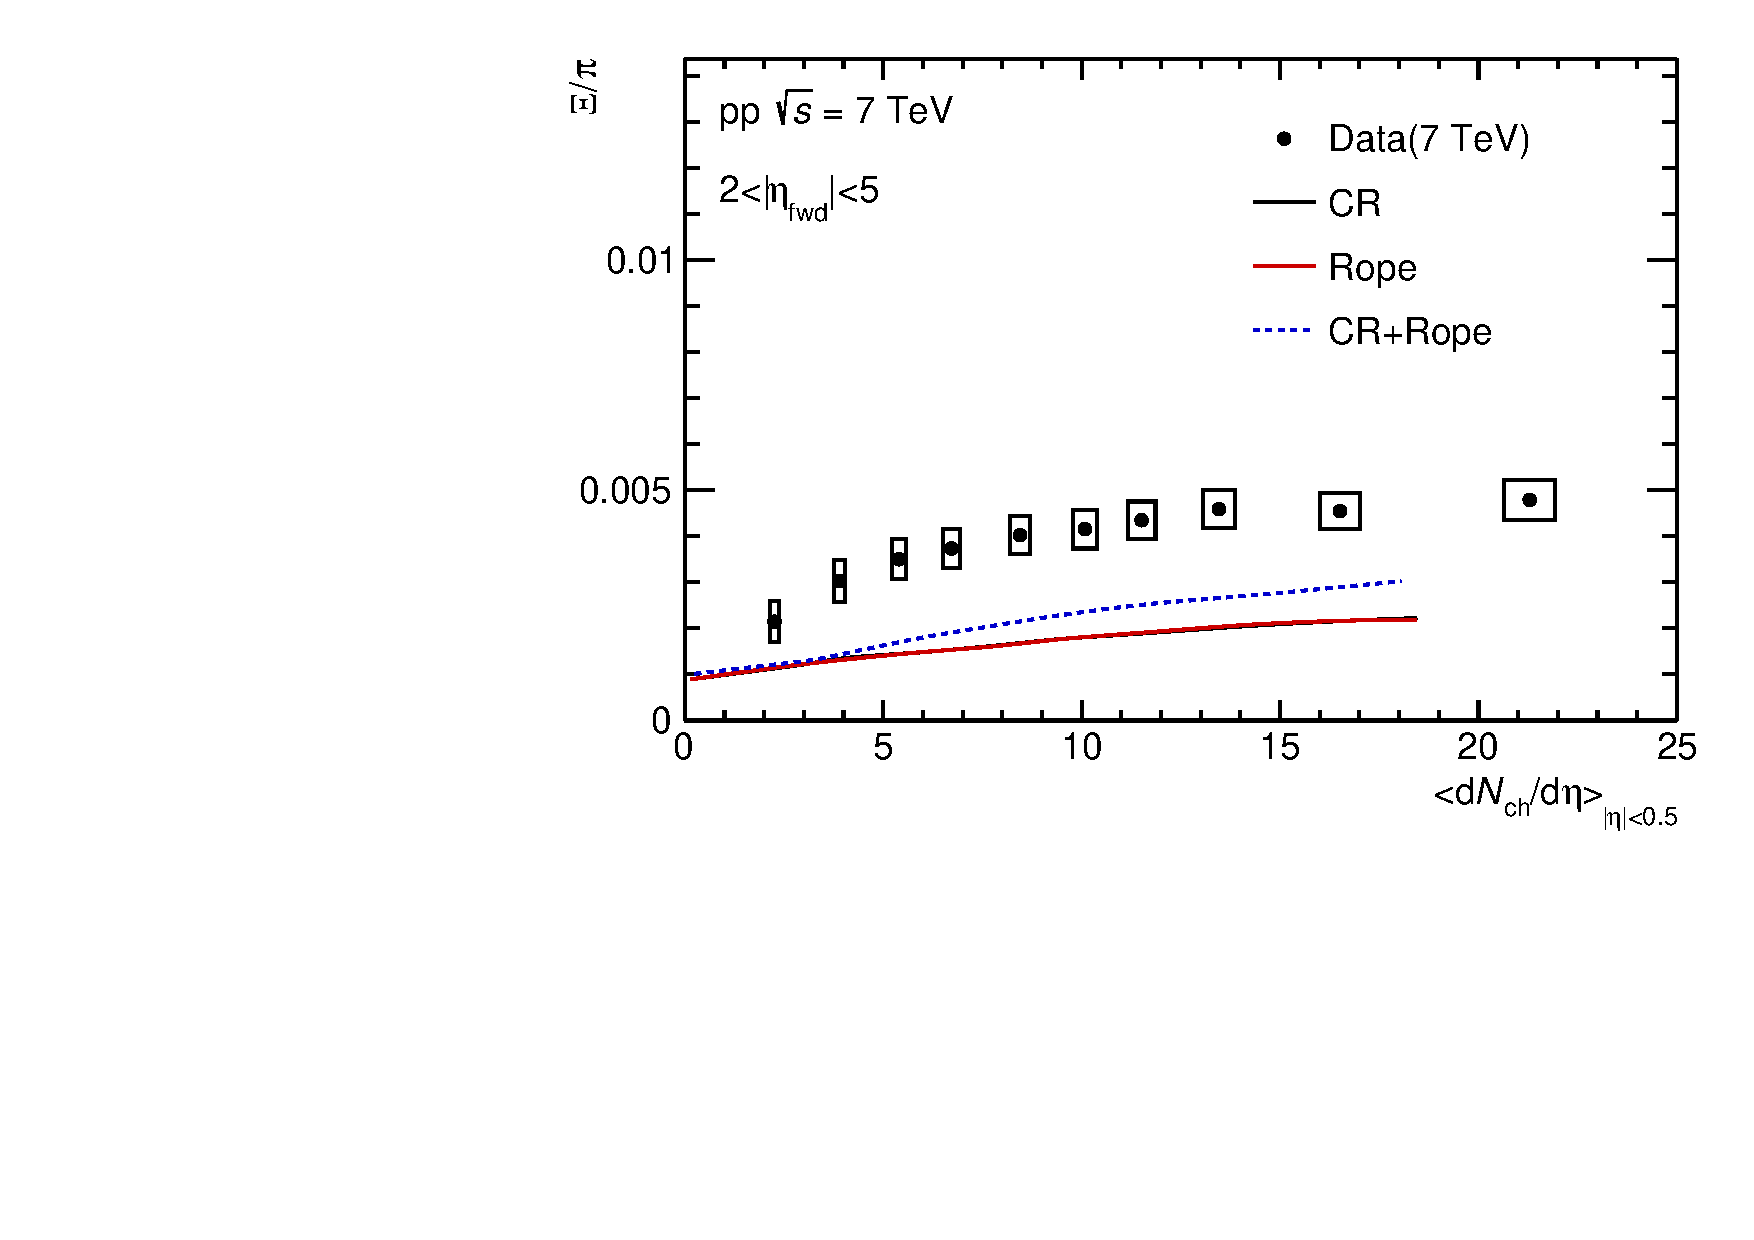
\includegraphics[width=.48\textwidth]{Xi_PiRatio}
		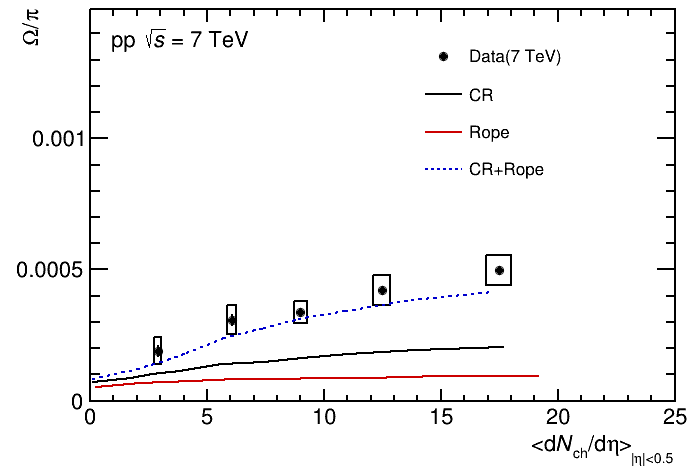
\includegraphics[width=.48\textwidth]{Omega_PiRatio}
	\end{center}
	\caption{Inclusive integrated yields ratios of strange particle to $\pi$ with $\avdndeta$. (Data taken from arXiv:1606.07424v2)}
	\label{fig:InclIntePartoPiRatio}
\end{figure}

\begin{figure}[ht]
	\begin{center}
		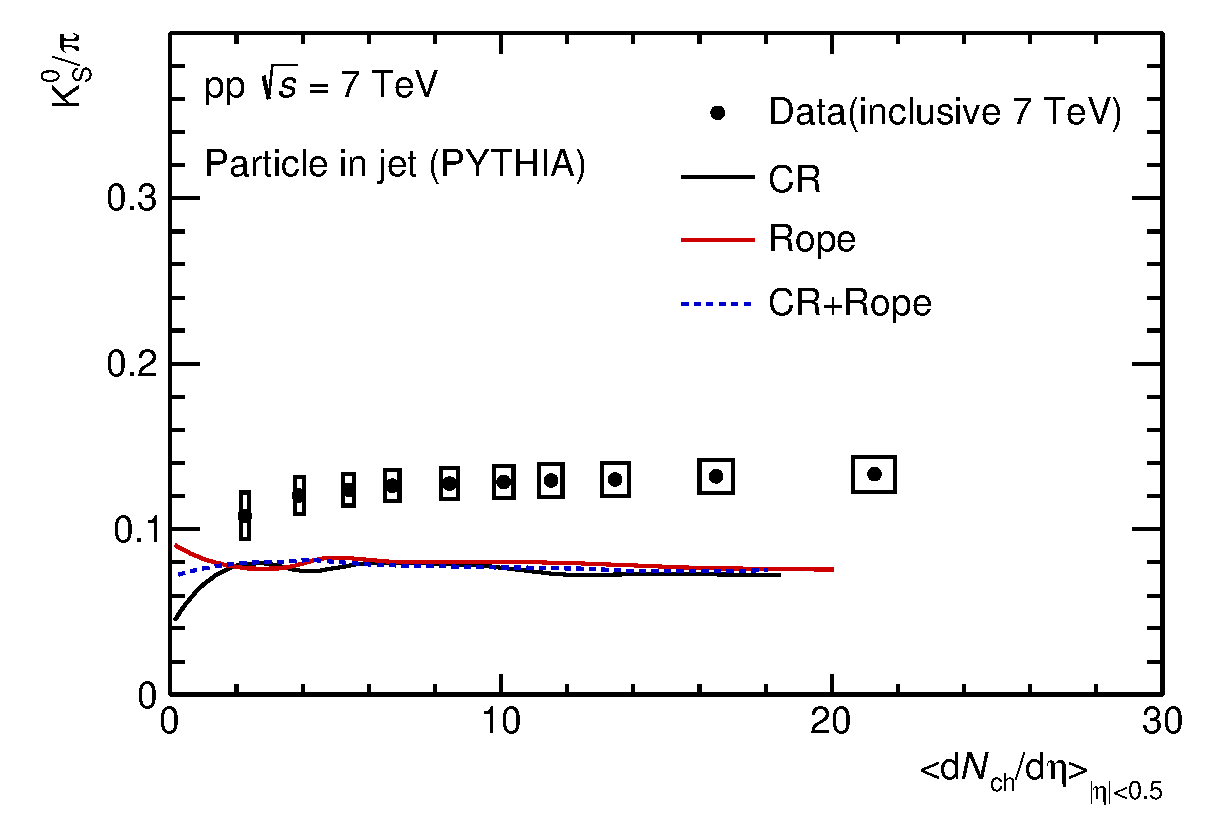
\includegraphics[width=.48\textwidth]{Kshort_PiRatio_JE}
		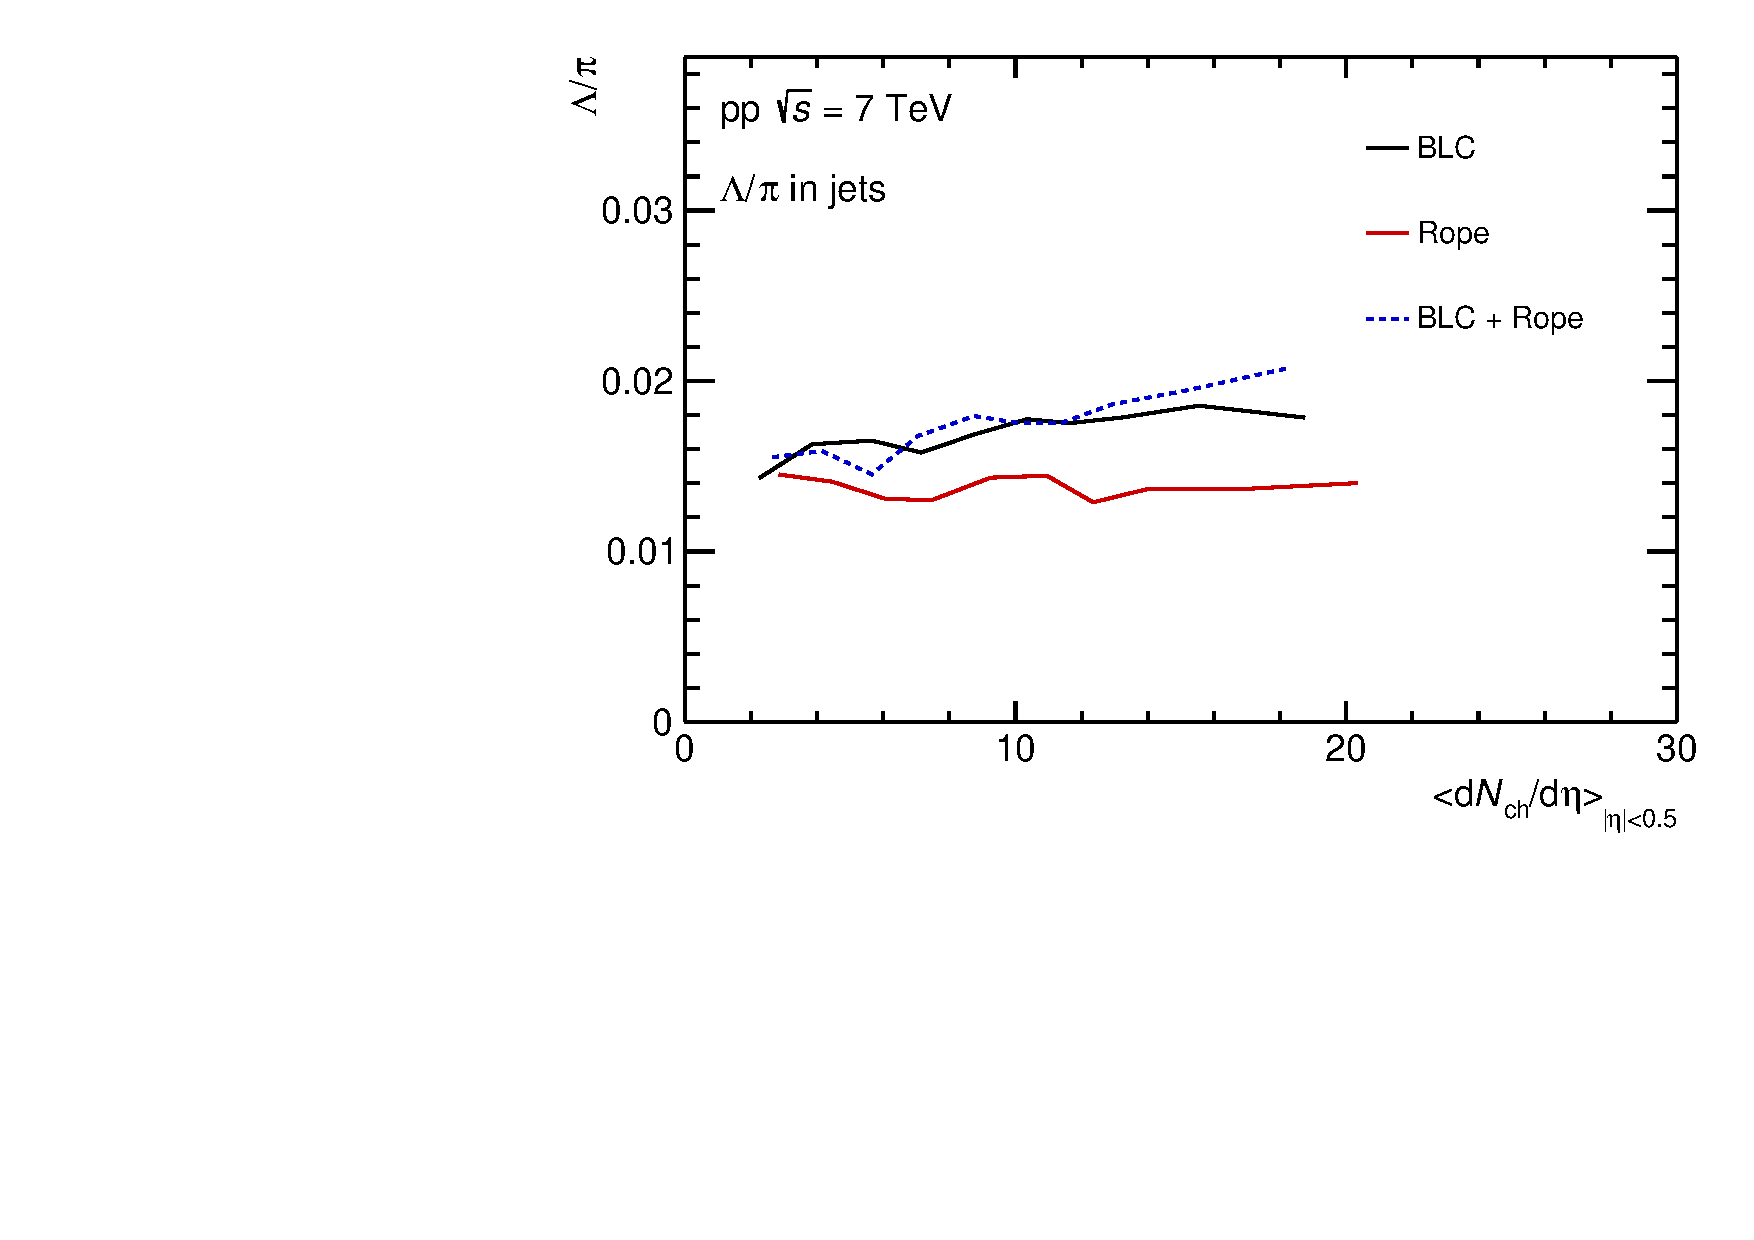
\includegraphics[width=.48\textwidth]{Lambda_PiRatio_JE}
		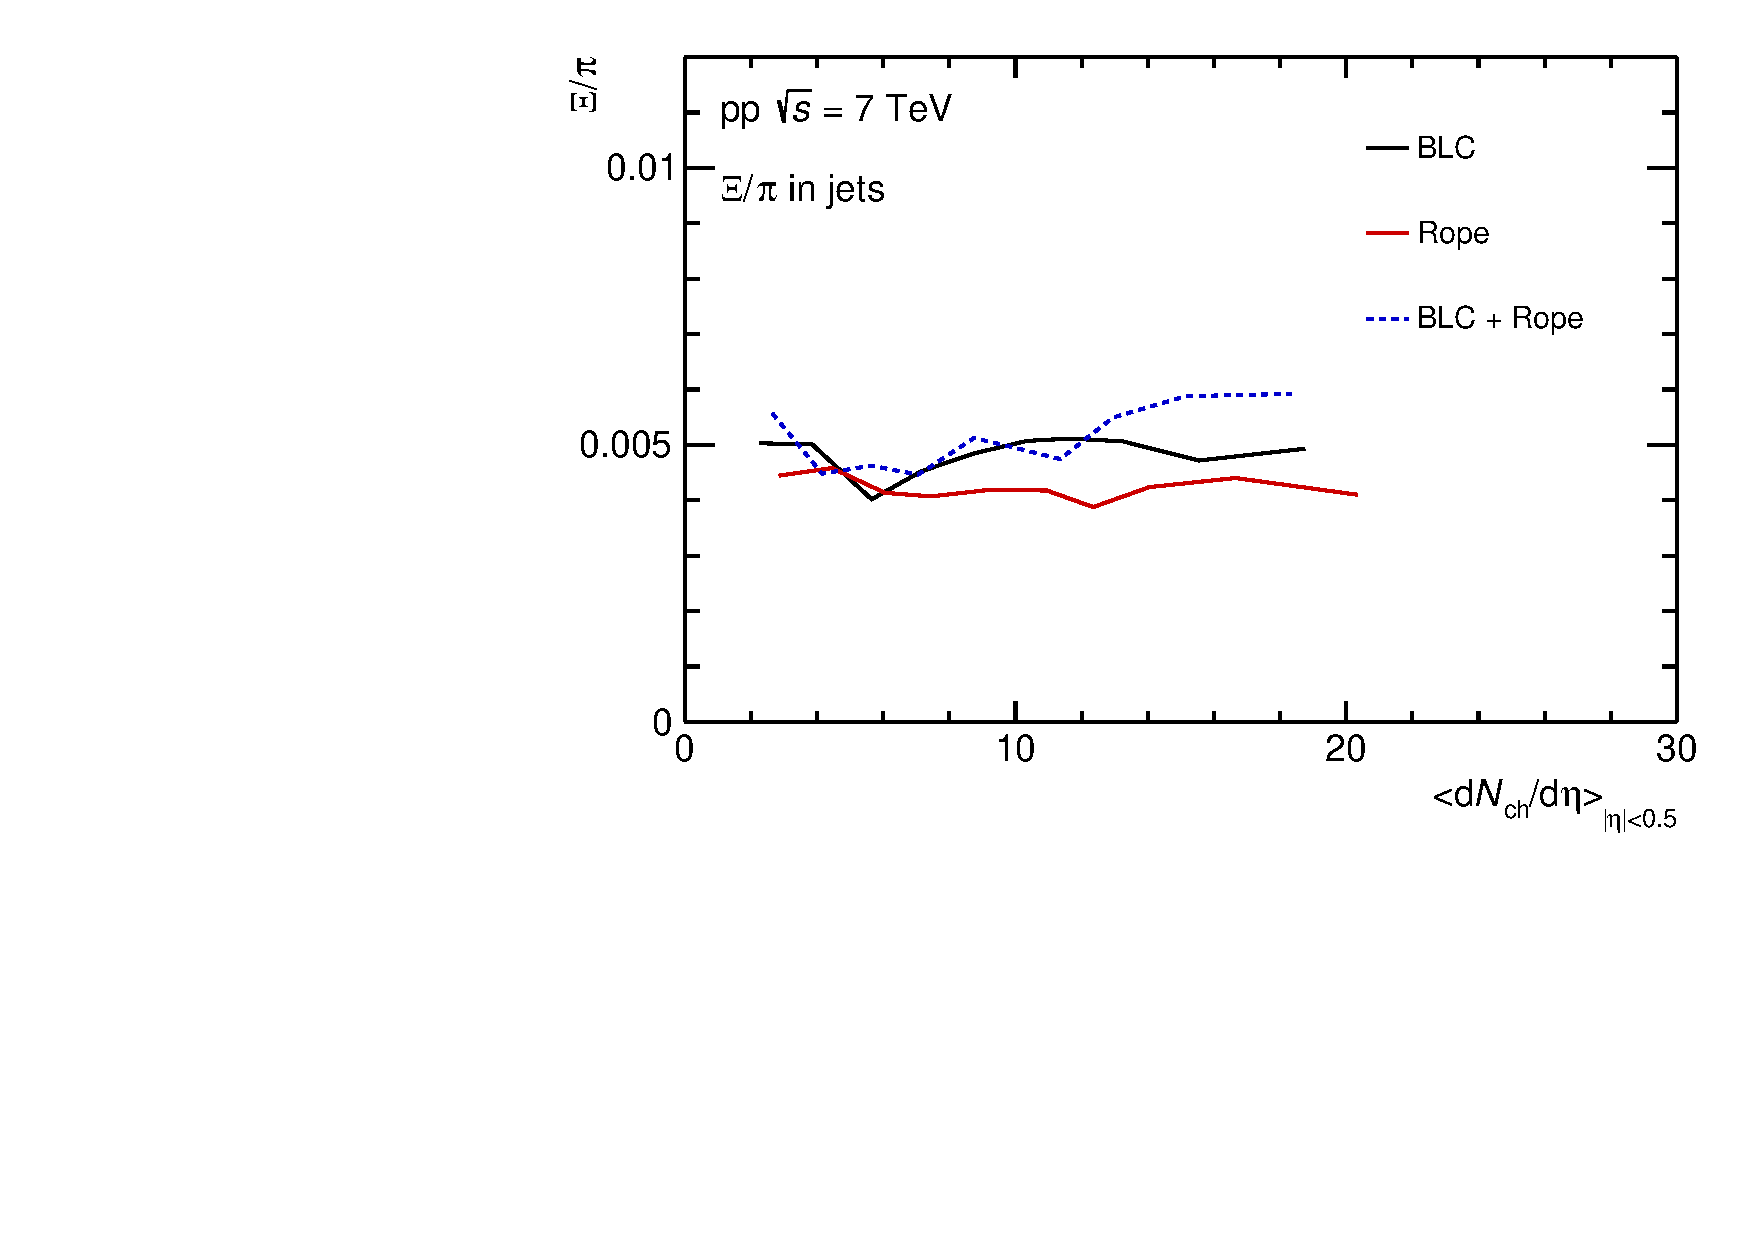
\includegraphics[width=.48\textwidth]{Xi_PiRatio_JE}
		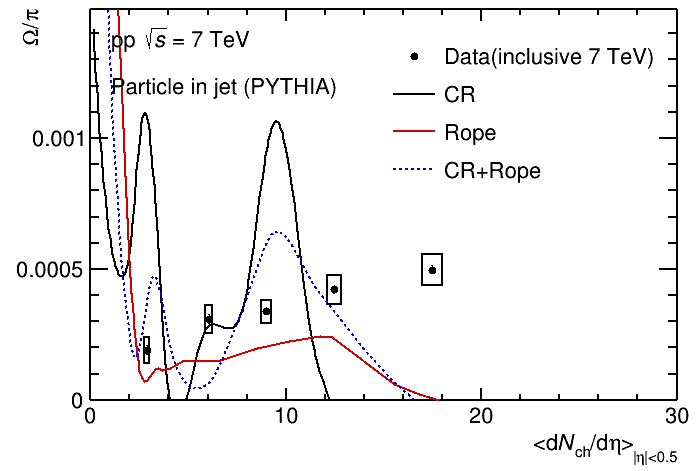
\includegraphics[width=.48\textwidth]{Omega_PiRatio_JE}
	\end{center}
	\caption{Integrated yields ratios in jet of strange particle to $\pi$ with $\avdndeta$.}
	\label{fig:JEIntePartoPiRatio}
\end{figure}


\begin{figure}[ht]
        \begin{center}
                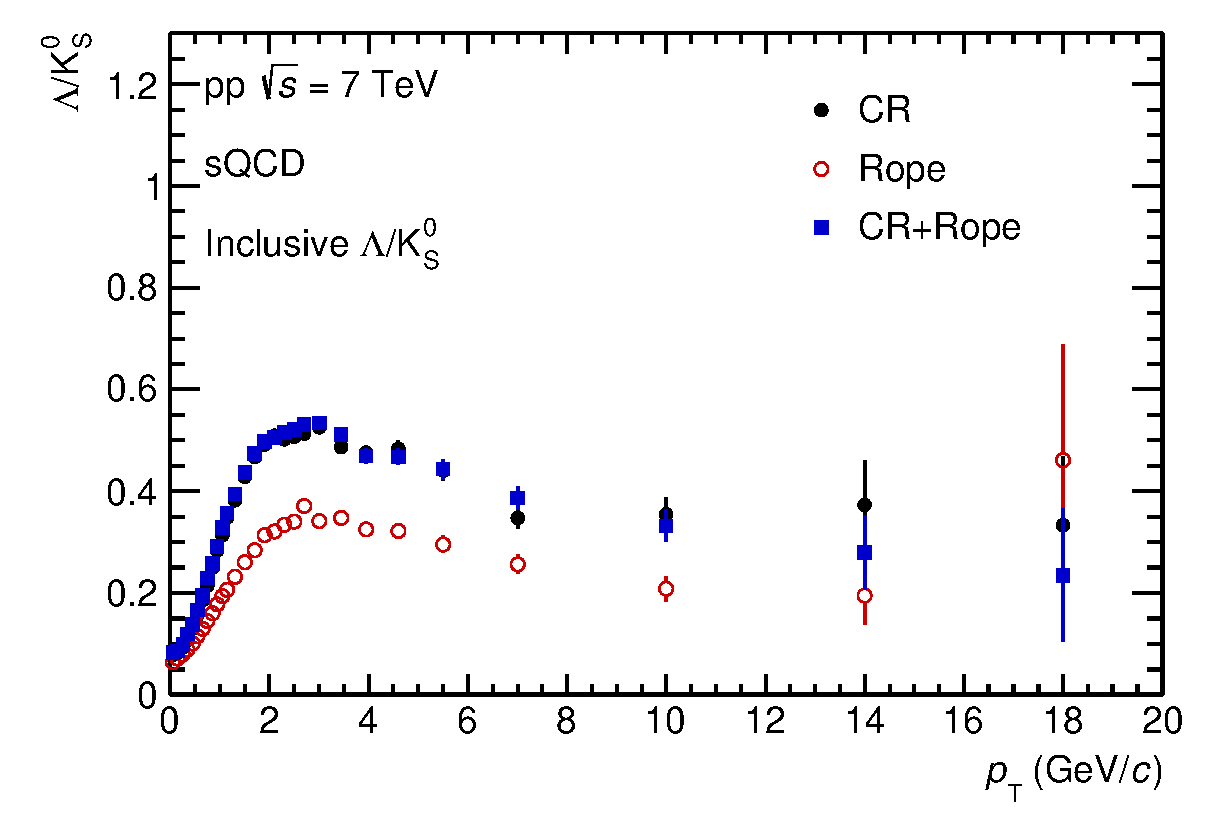
\includegraphics[width=.32\textwidth]{LKRatio_Incl}
                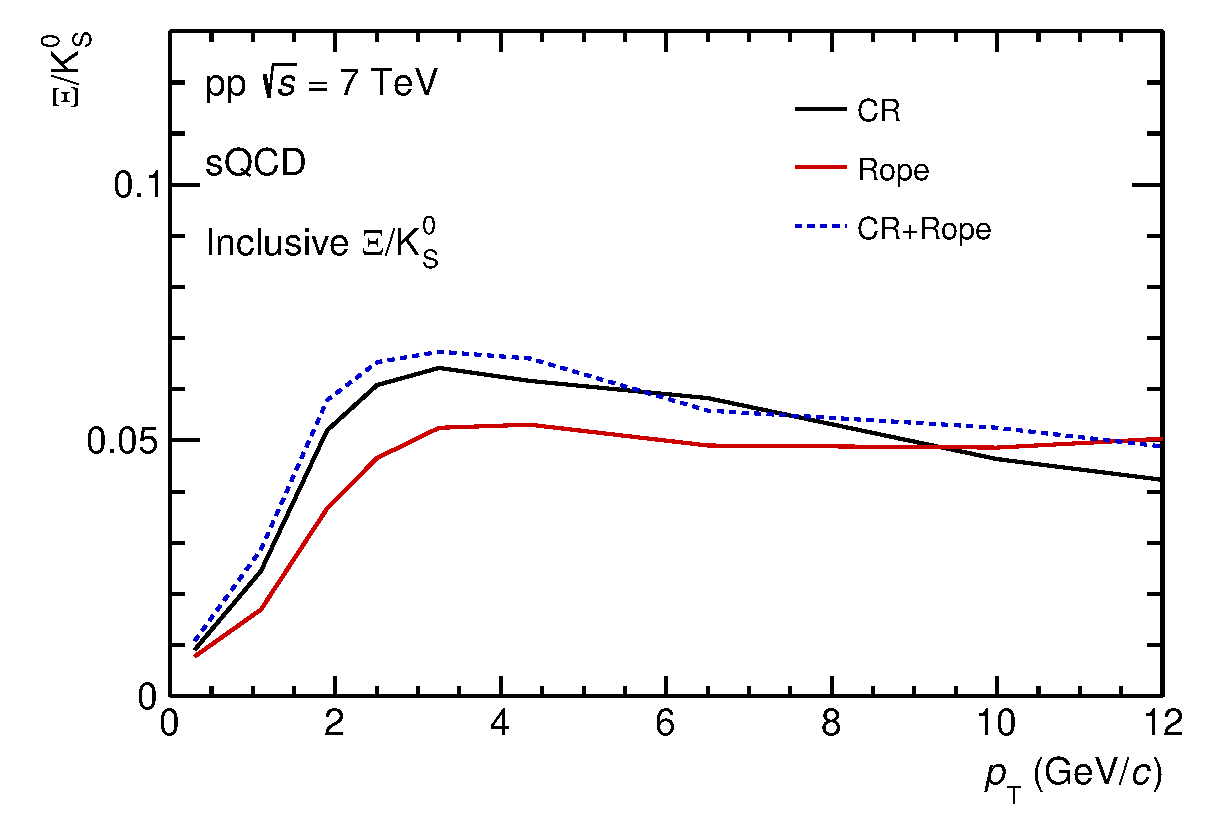
\includegraphics[width=.32\textwidth]{XKRatio_Incl}
                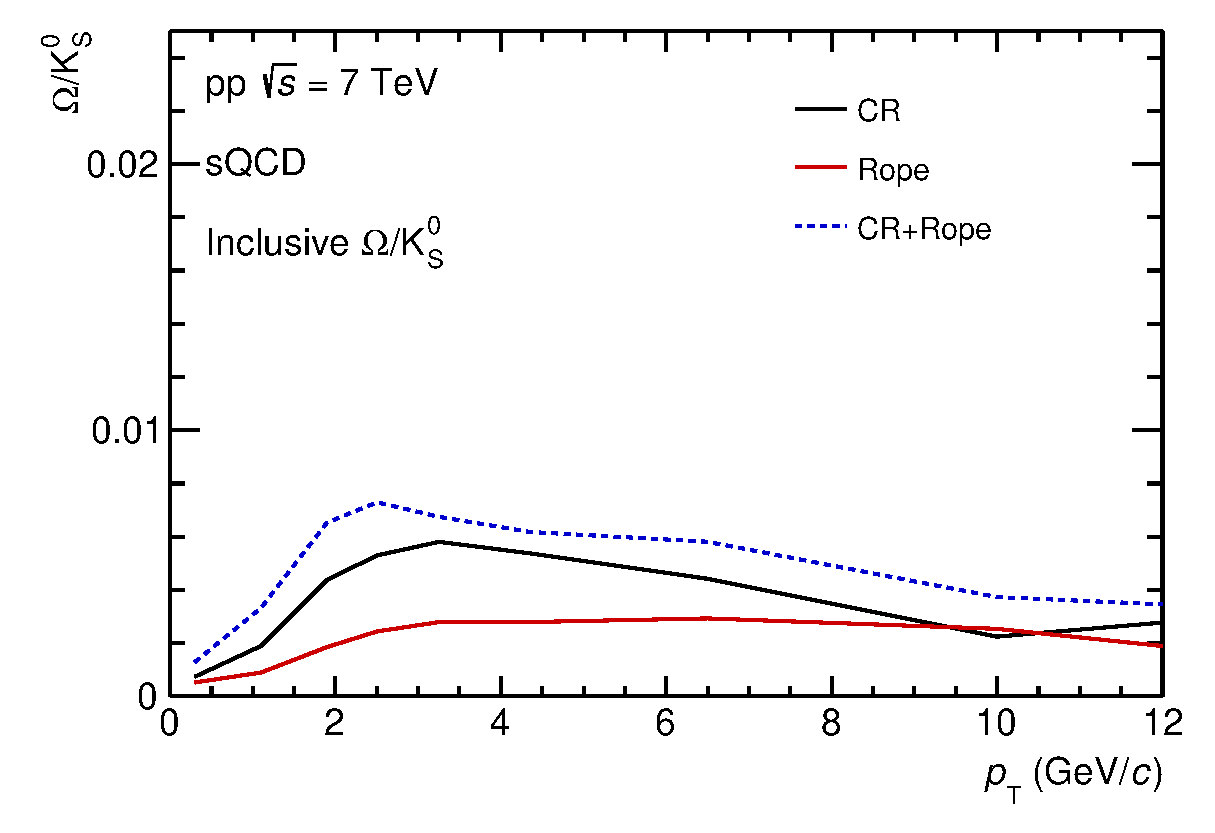
\includegraphics[width=.32\textwidth]{OKRatio_Incl}
                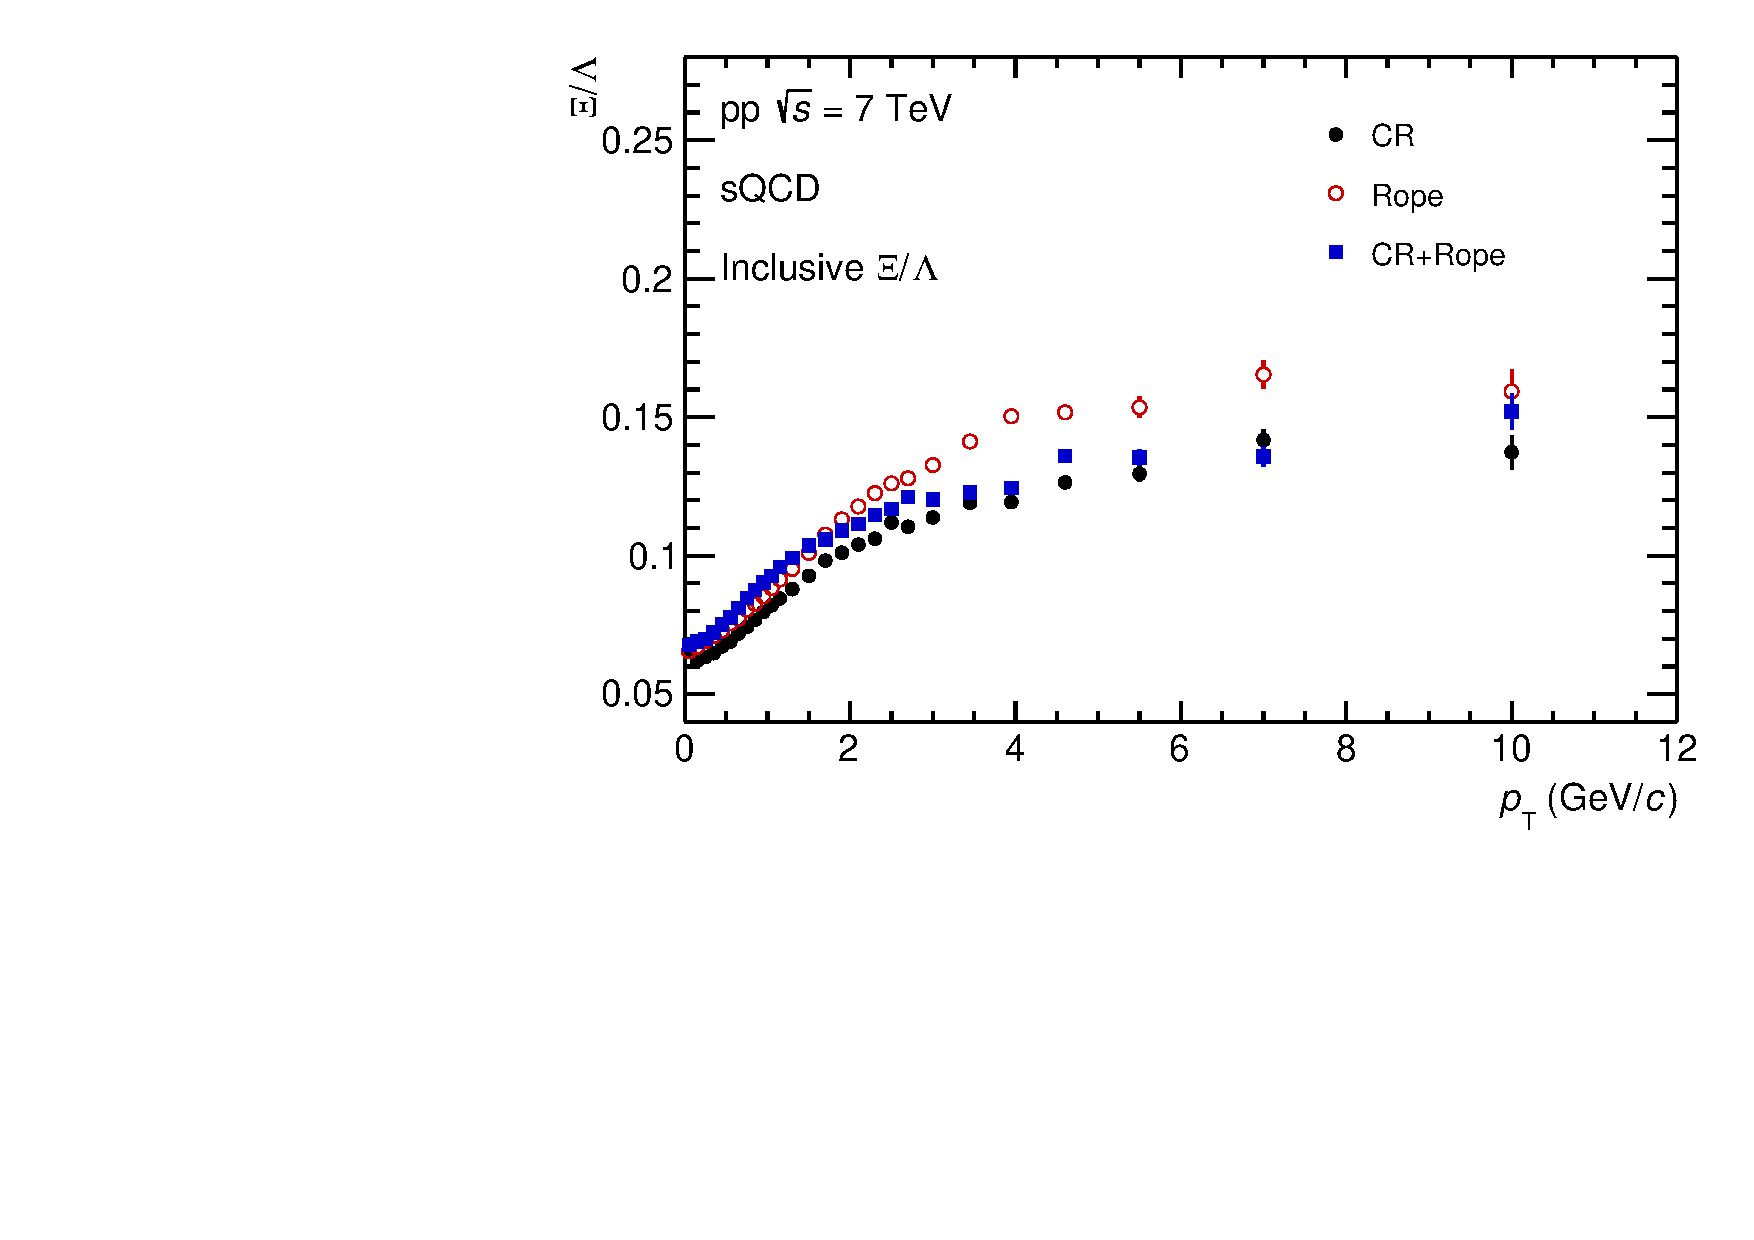
\includegraphics[width=.32\textwidth]{XLRatio_Incl}
                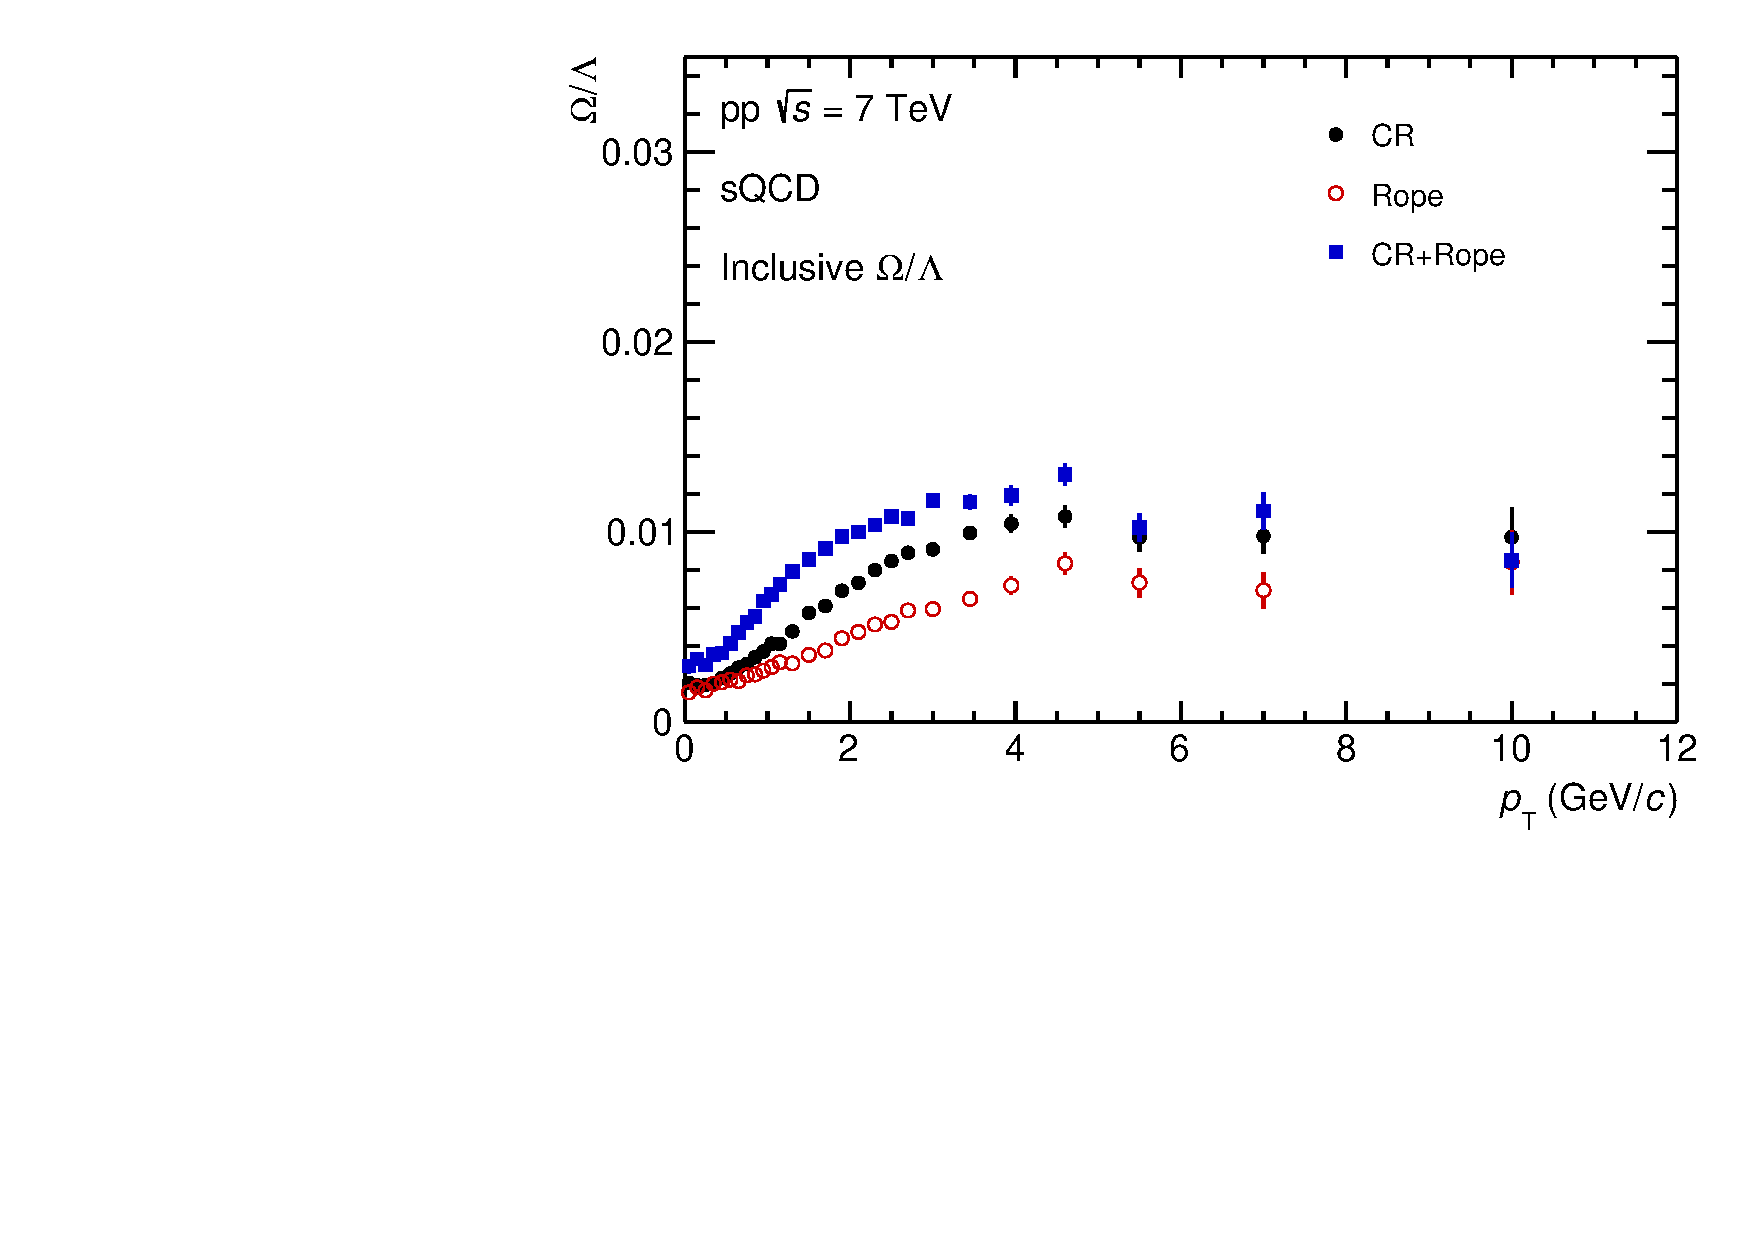
\includegraphics[width=.32\textwidth]{OLRatio_Incl}
                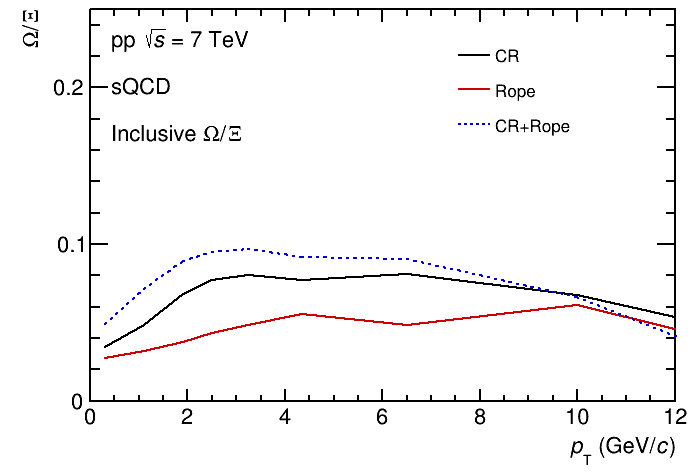
\includegraphics[width=.32\textwidth]{OXRatio_Incl}
        \end{center}
	\caption{Inclusive baryon-to-meson ratio(top) and Baryon-to-meson ratio(bottom) with $\pT$ distribution. (Only find data point of Lambda/Kshort in 13 TeV from arXiv:2005.11120)}
        \label{fig:InclParRatio}
\end{figure}

\begin{figure}[ht]
        \begin{center}
                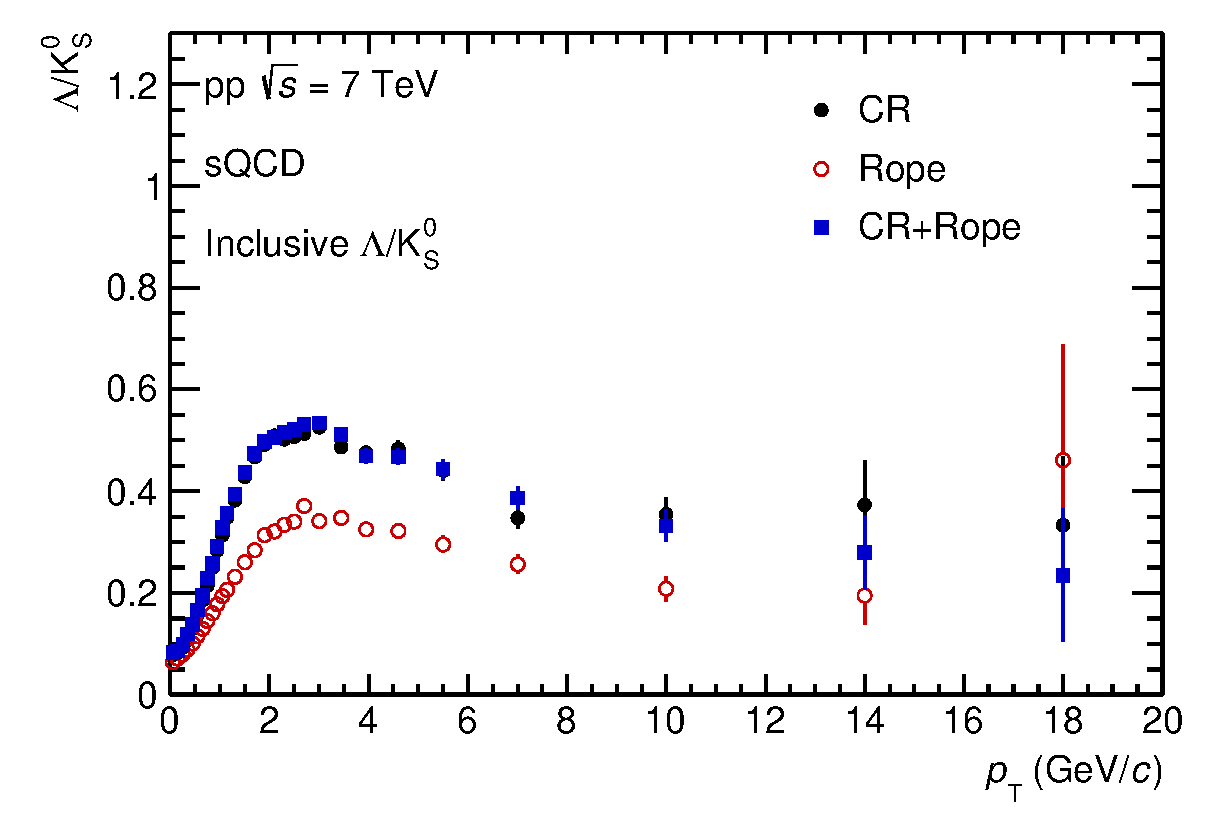
\includegraphics[width=.48\textwidth]{LKRatio_Incl}
                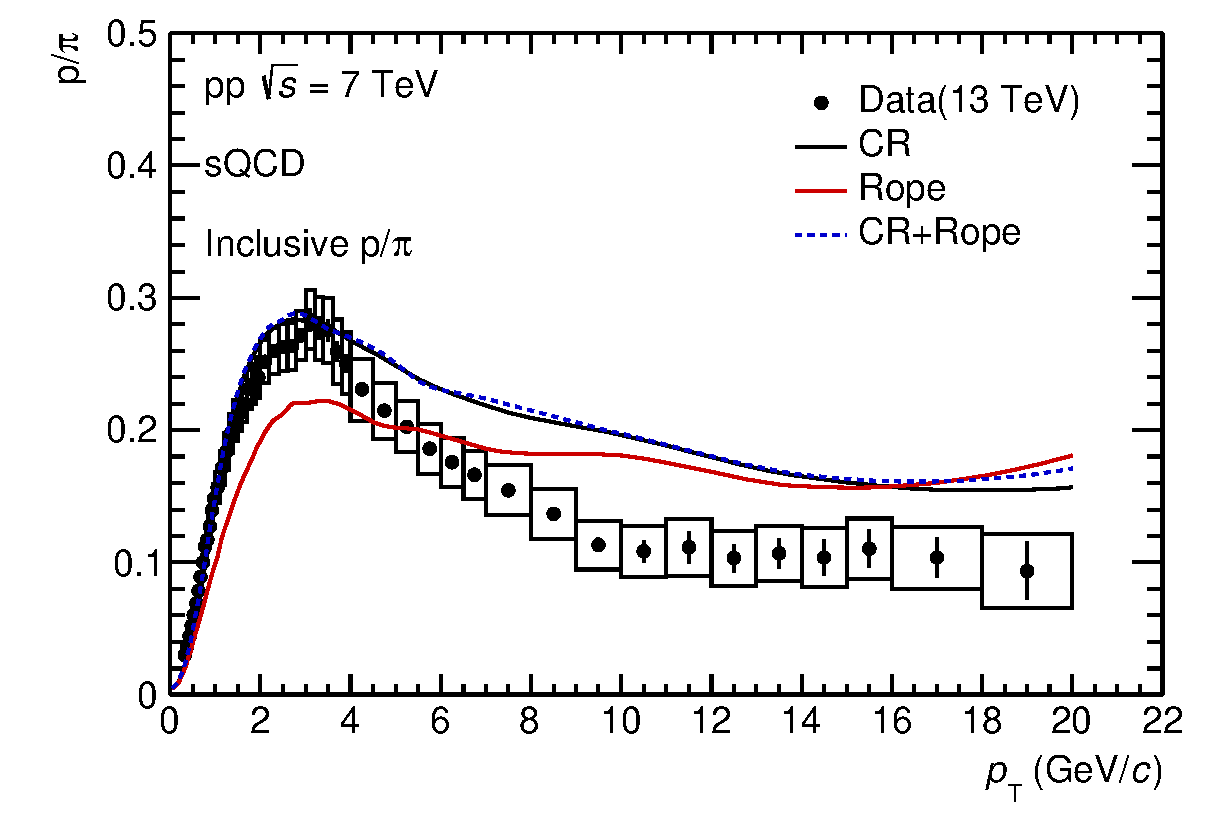
\includegraphics[width=.48\textwidth]{ProtonPionRatio_Incl}
                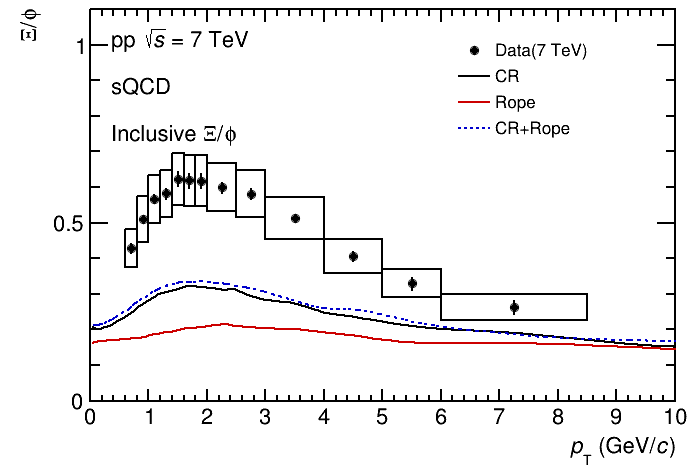
\includegraphics[width=.48\textwidth]{XiPhiRatio_Incl}
                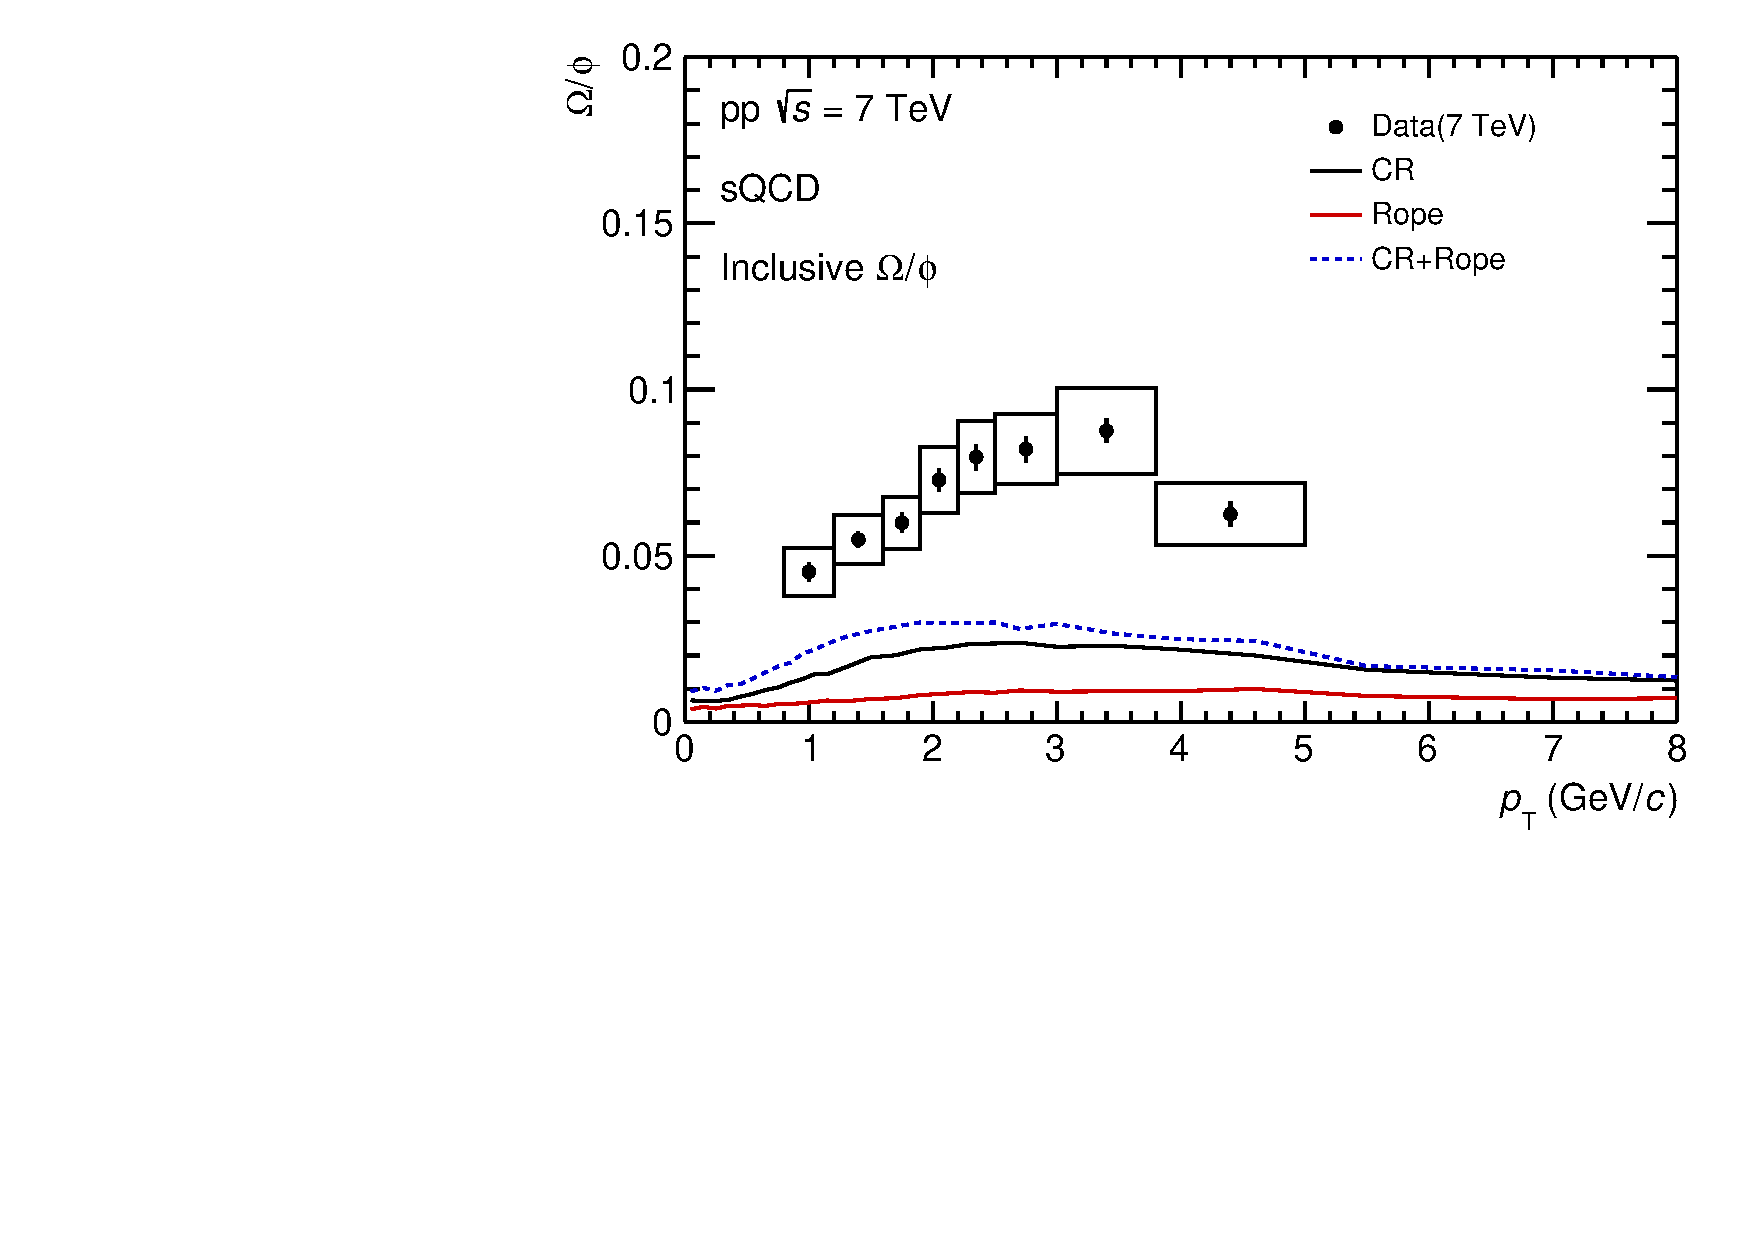
\includegraphics[width=.48\textwidth]{OmegaPhiRatio_Incl}
        \end{center}
	\caption{Inclusive baryon-to-meson ratio(top) with $\pT$ distribution.}
        \label{fig:InclBtMratio}
\end{figure}

\begin{figure}[ht]
        \begin{center}
                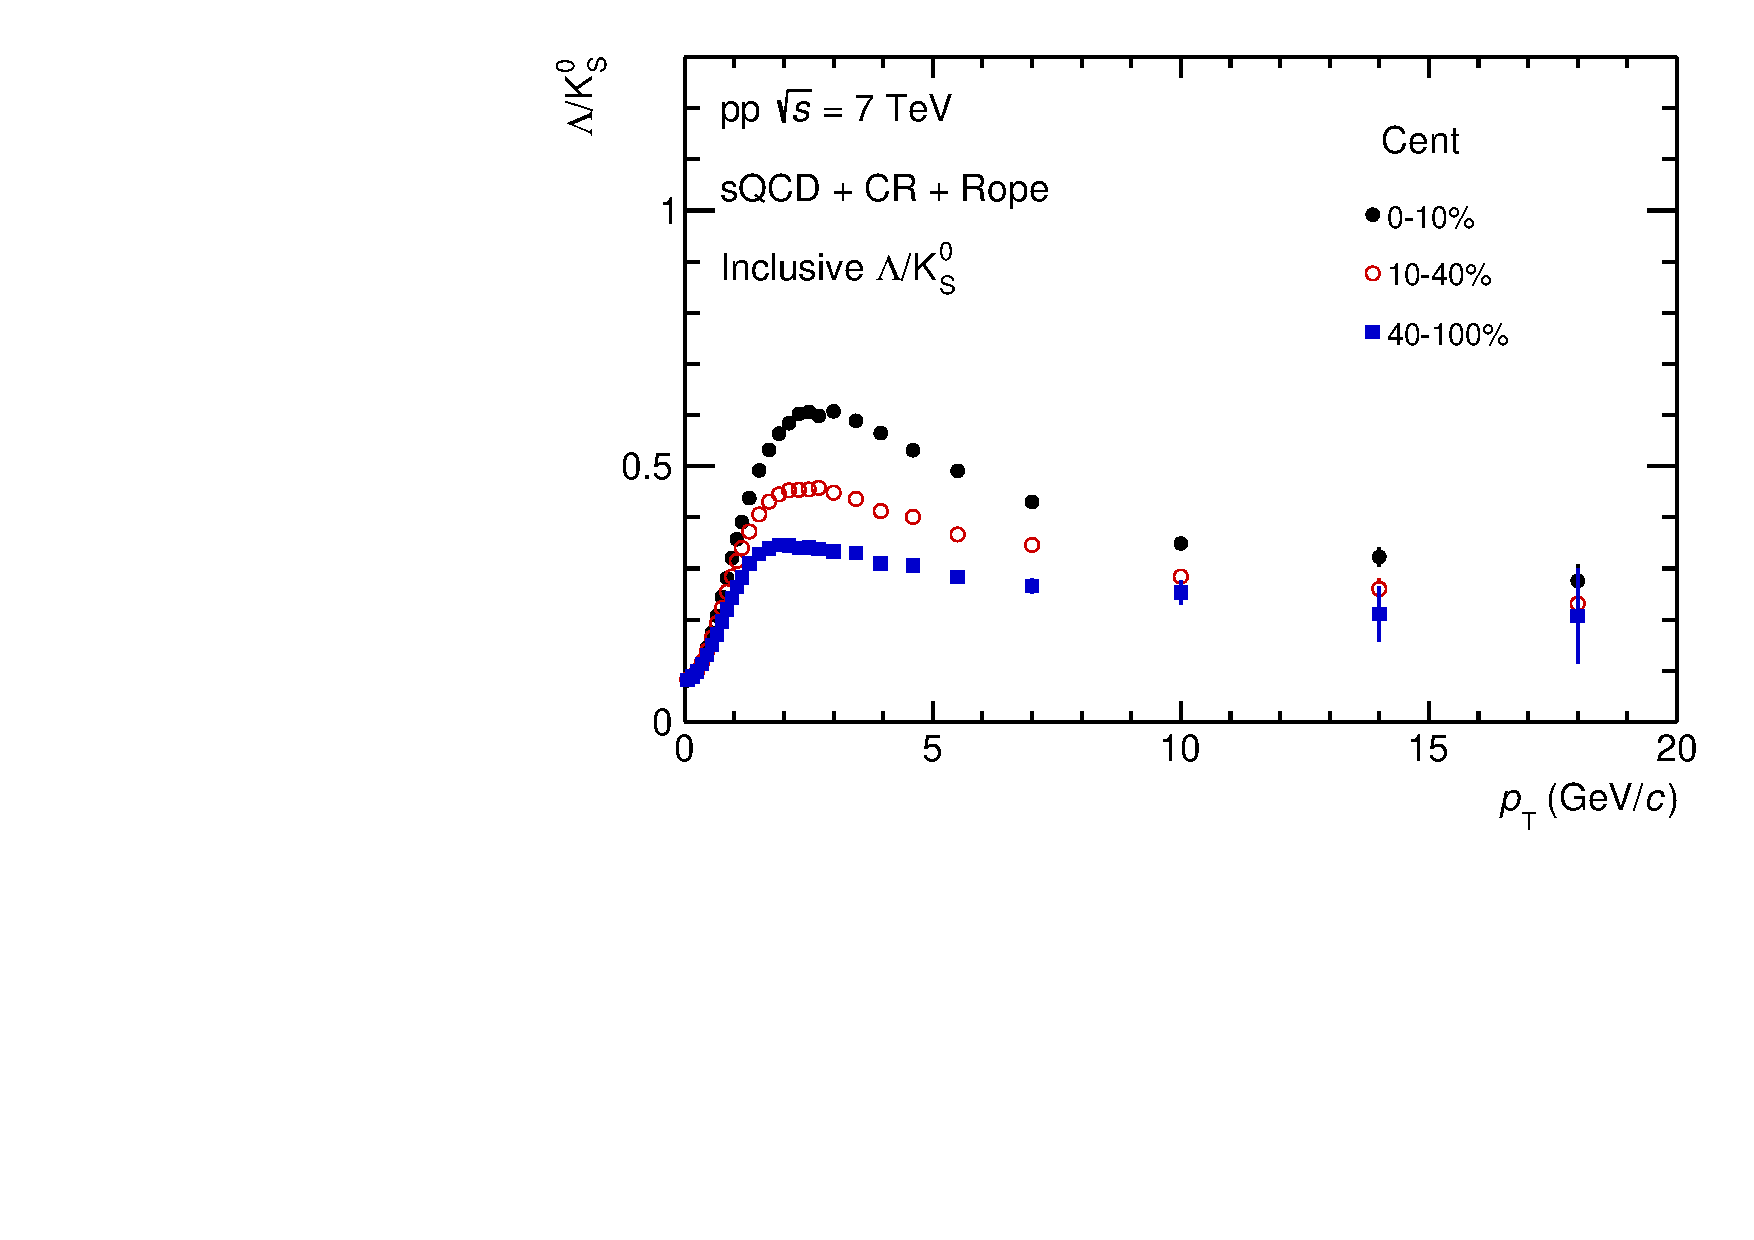
\includegraphics[width=.32\textwidth]{LKRatio_Incl_Cent_cr_rope}
                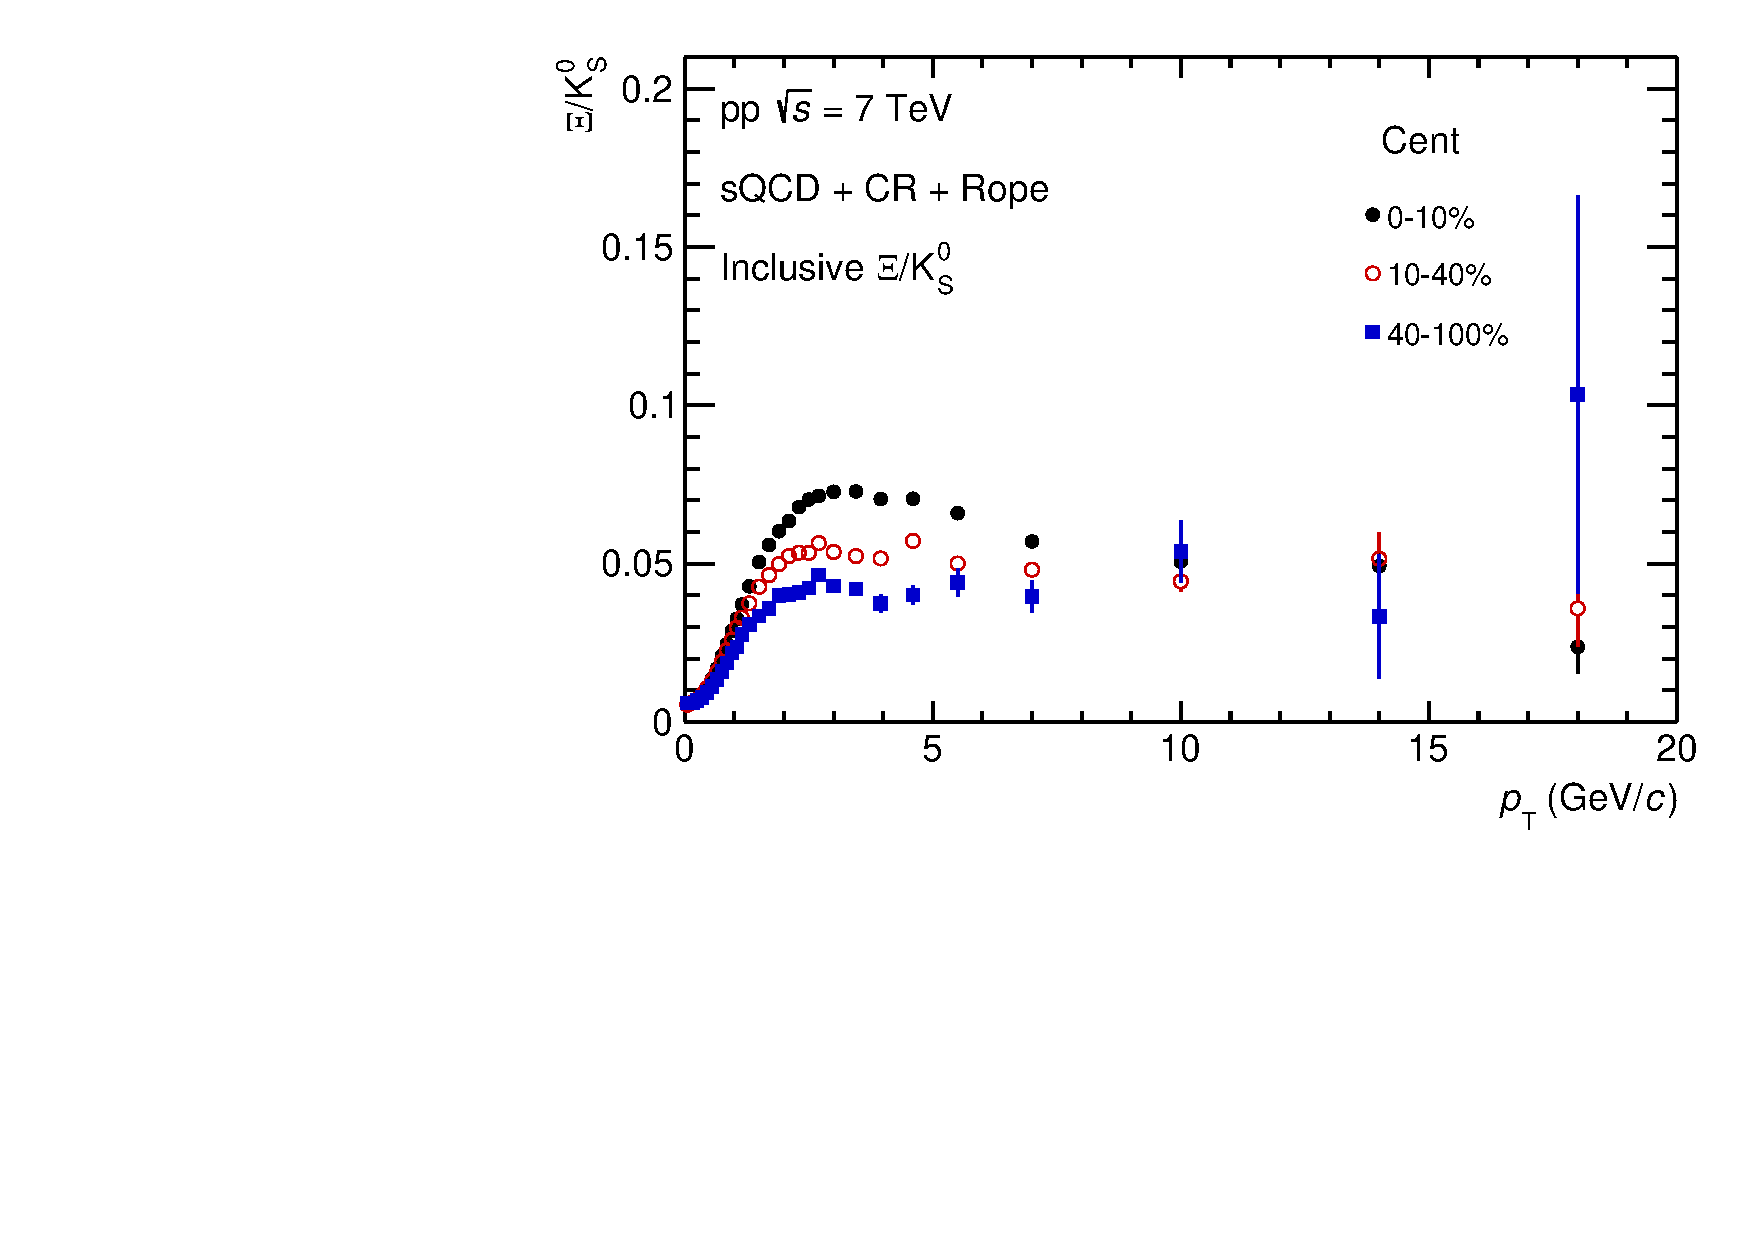
\includegraphics[width=.32\textwidth]{XKRatio_Incl_Cent_cr_rope}
                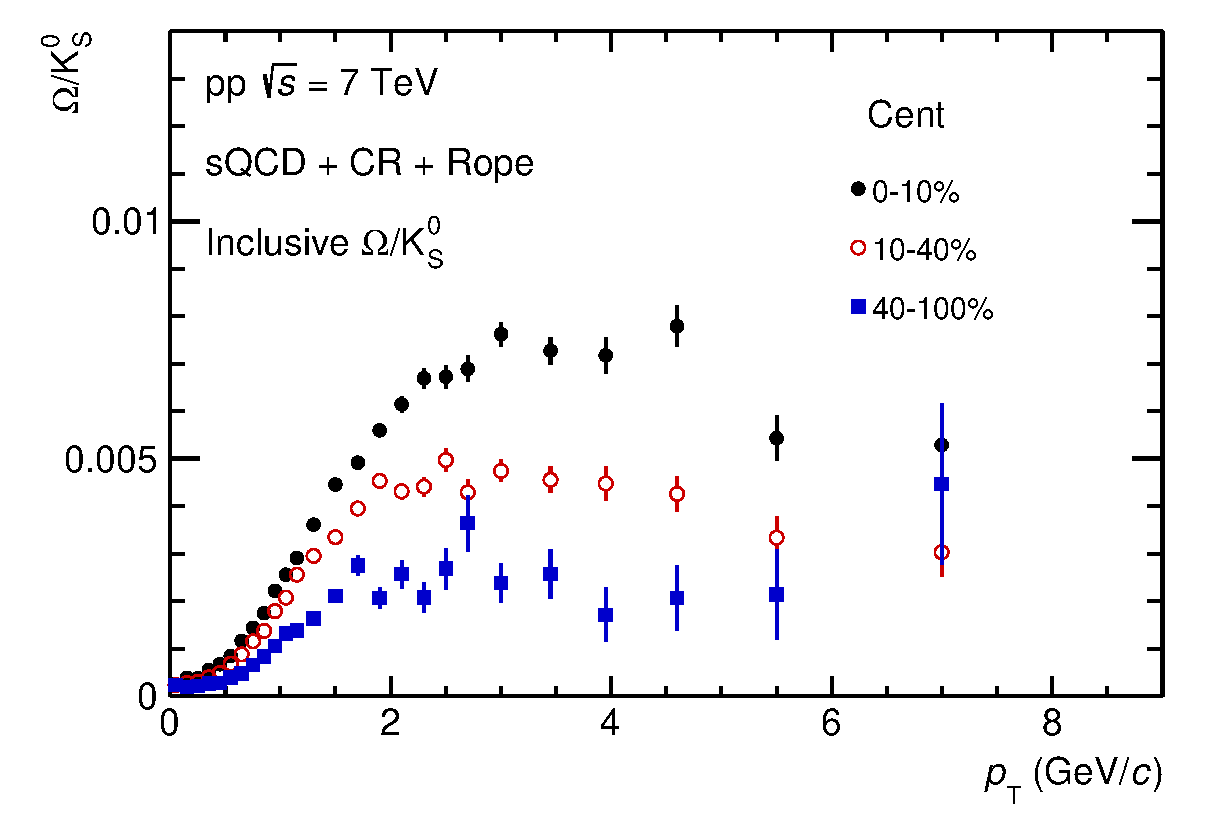
\includegraphics[width=.32\textwidth]{OKRatio_Incl_Cent_cr_rope}
                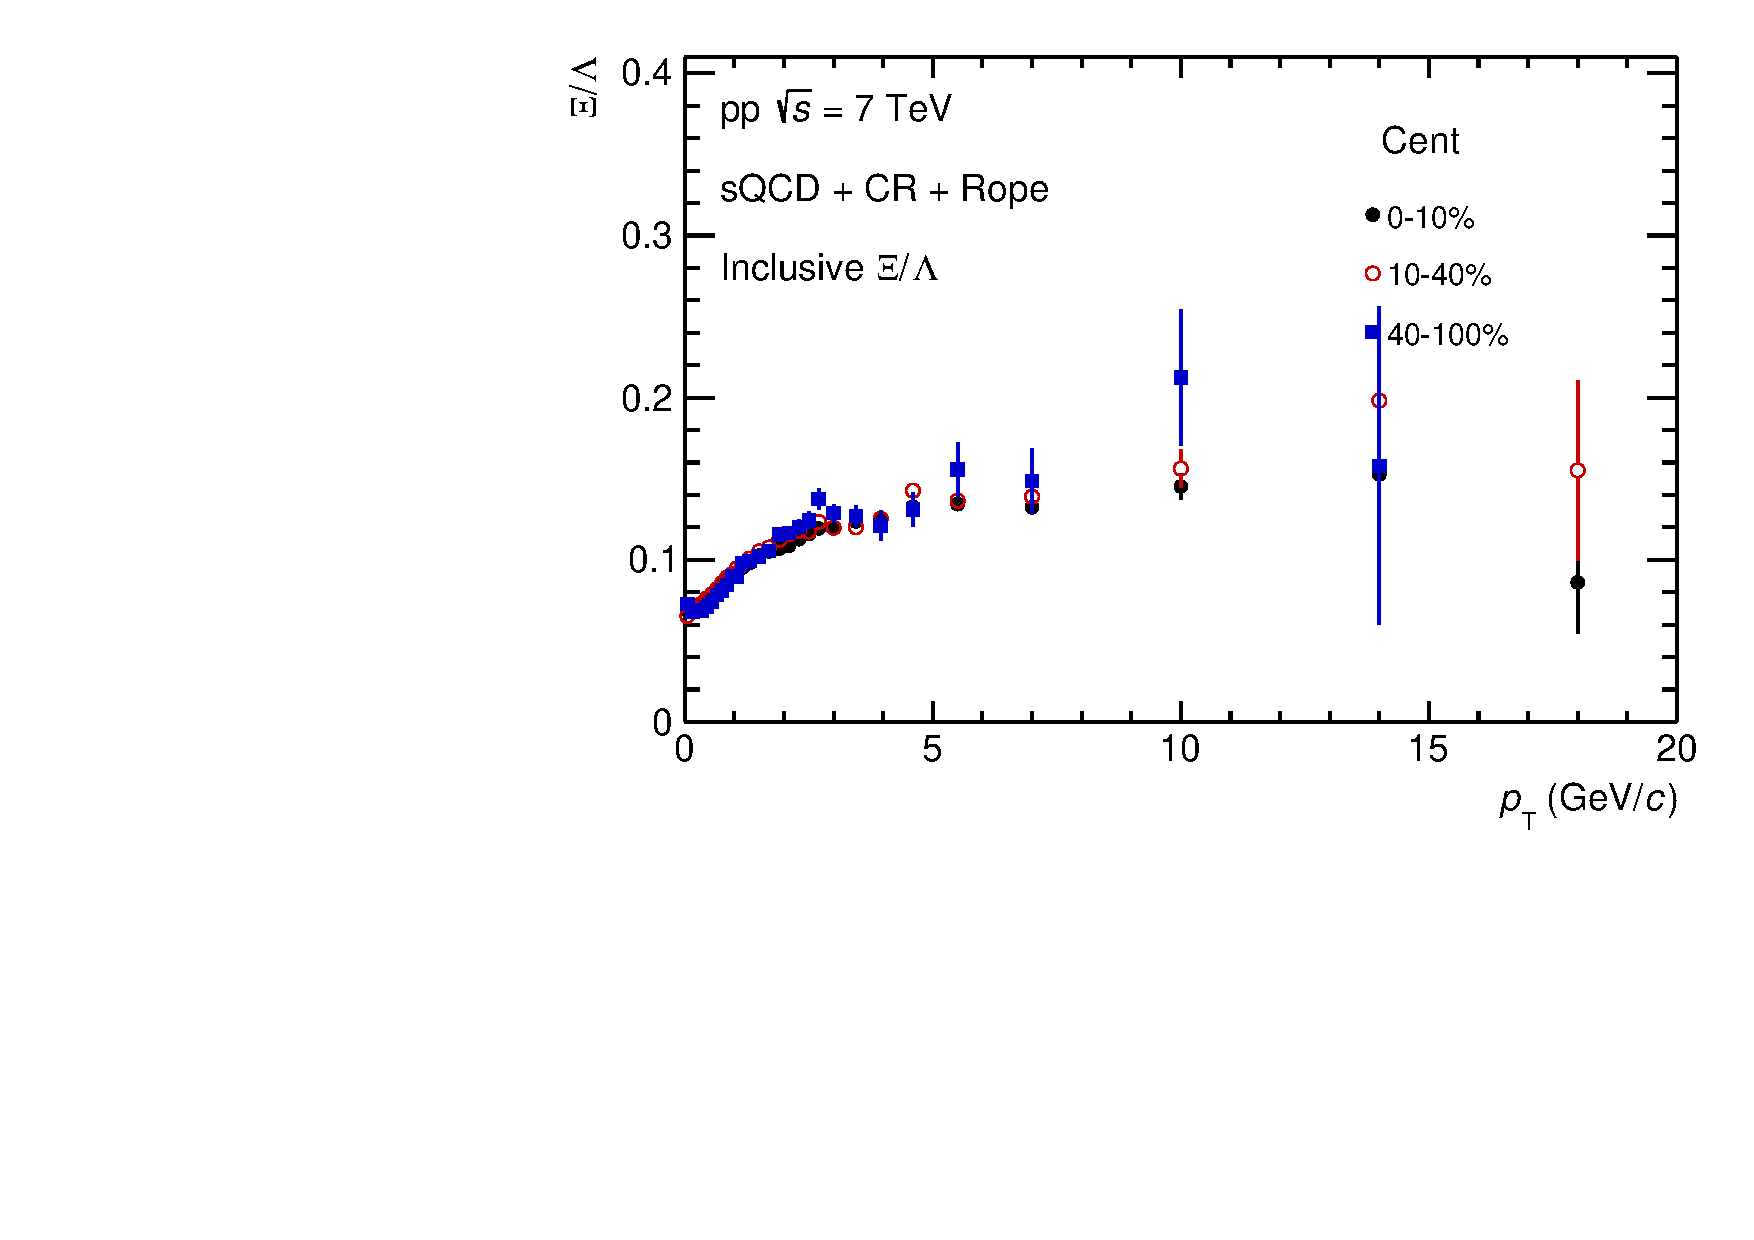
\includegraphics[width=.32\textwidth]{XLRatio_Incl_Cent_cr_rope}
                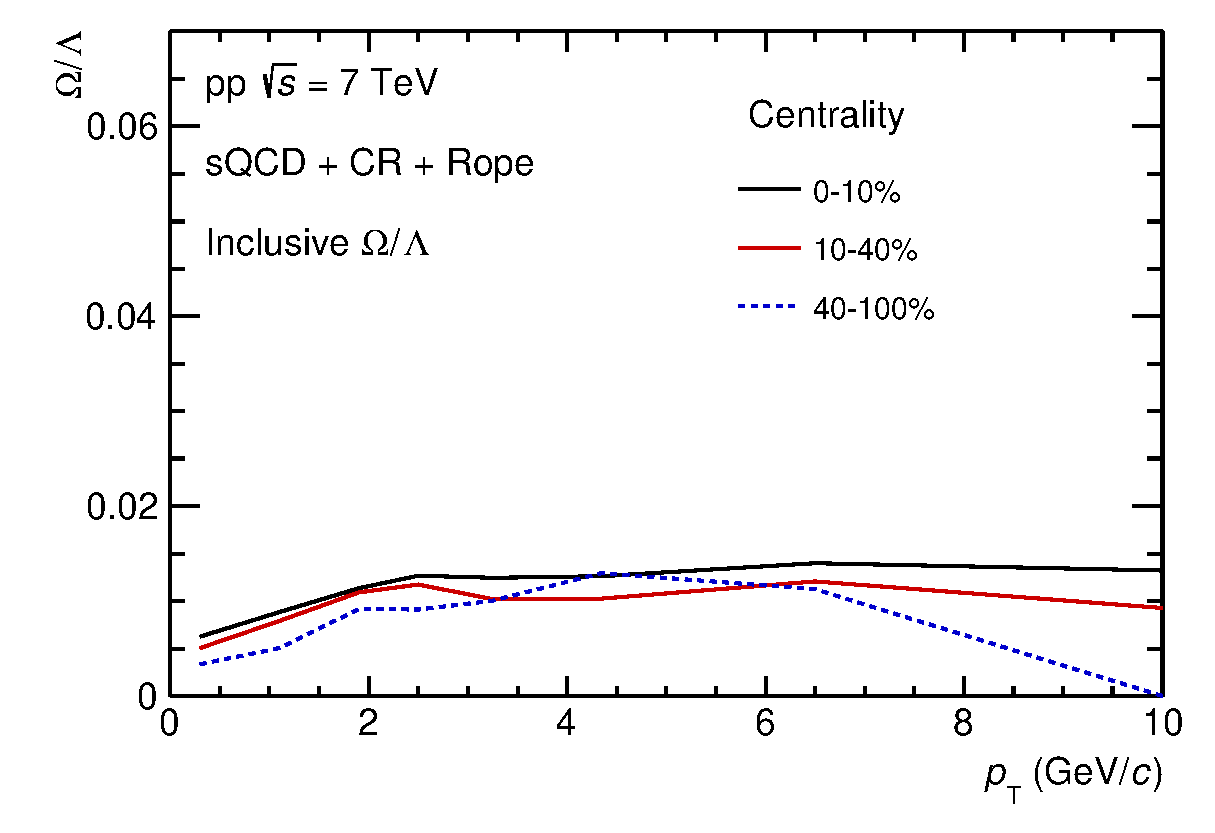
\includegraphics[width=.32\textwidth]{OLRatio_Incl_Cent_cr_rope}
                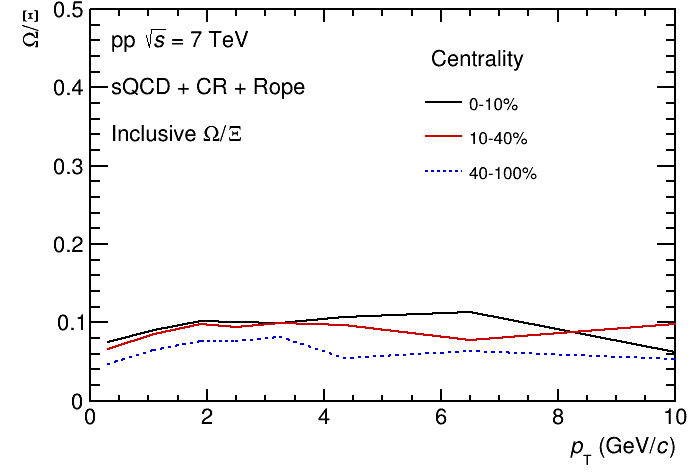
\includegraphics[width=.32\textwidth]{OXRatio_Incl_Cent_cr_rope}
        \end{center}
	\caption{Baryon-to-meson ratio(top) and Baryon-to-meson ratio(bottom) with $\pT$ distribution in different centrality bins.}
        \label{fig:InclParRatioCent}
\end{figure}

\begin{figure}[ht]
        \begin{center}
                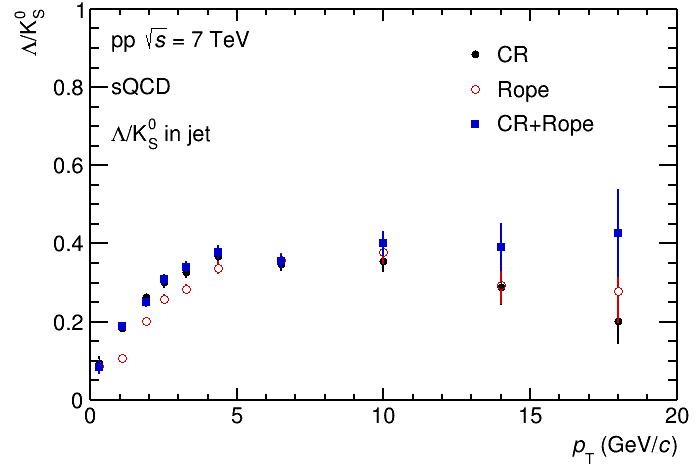
\includegraphics[width=.32\textwidth]{LKRatio_JE}
                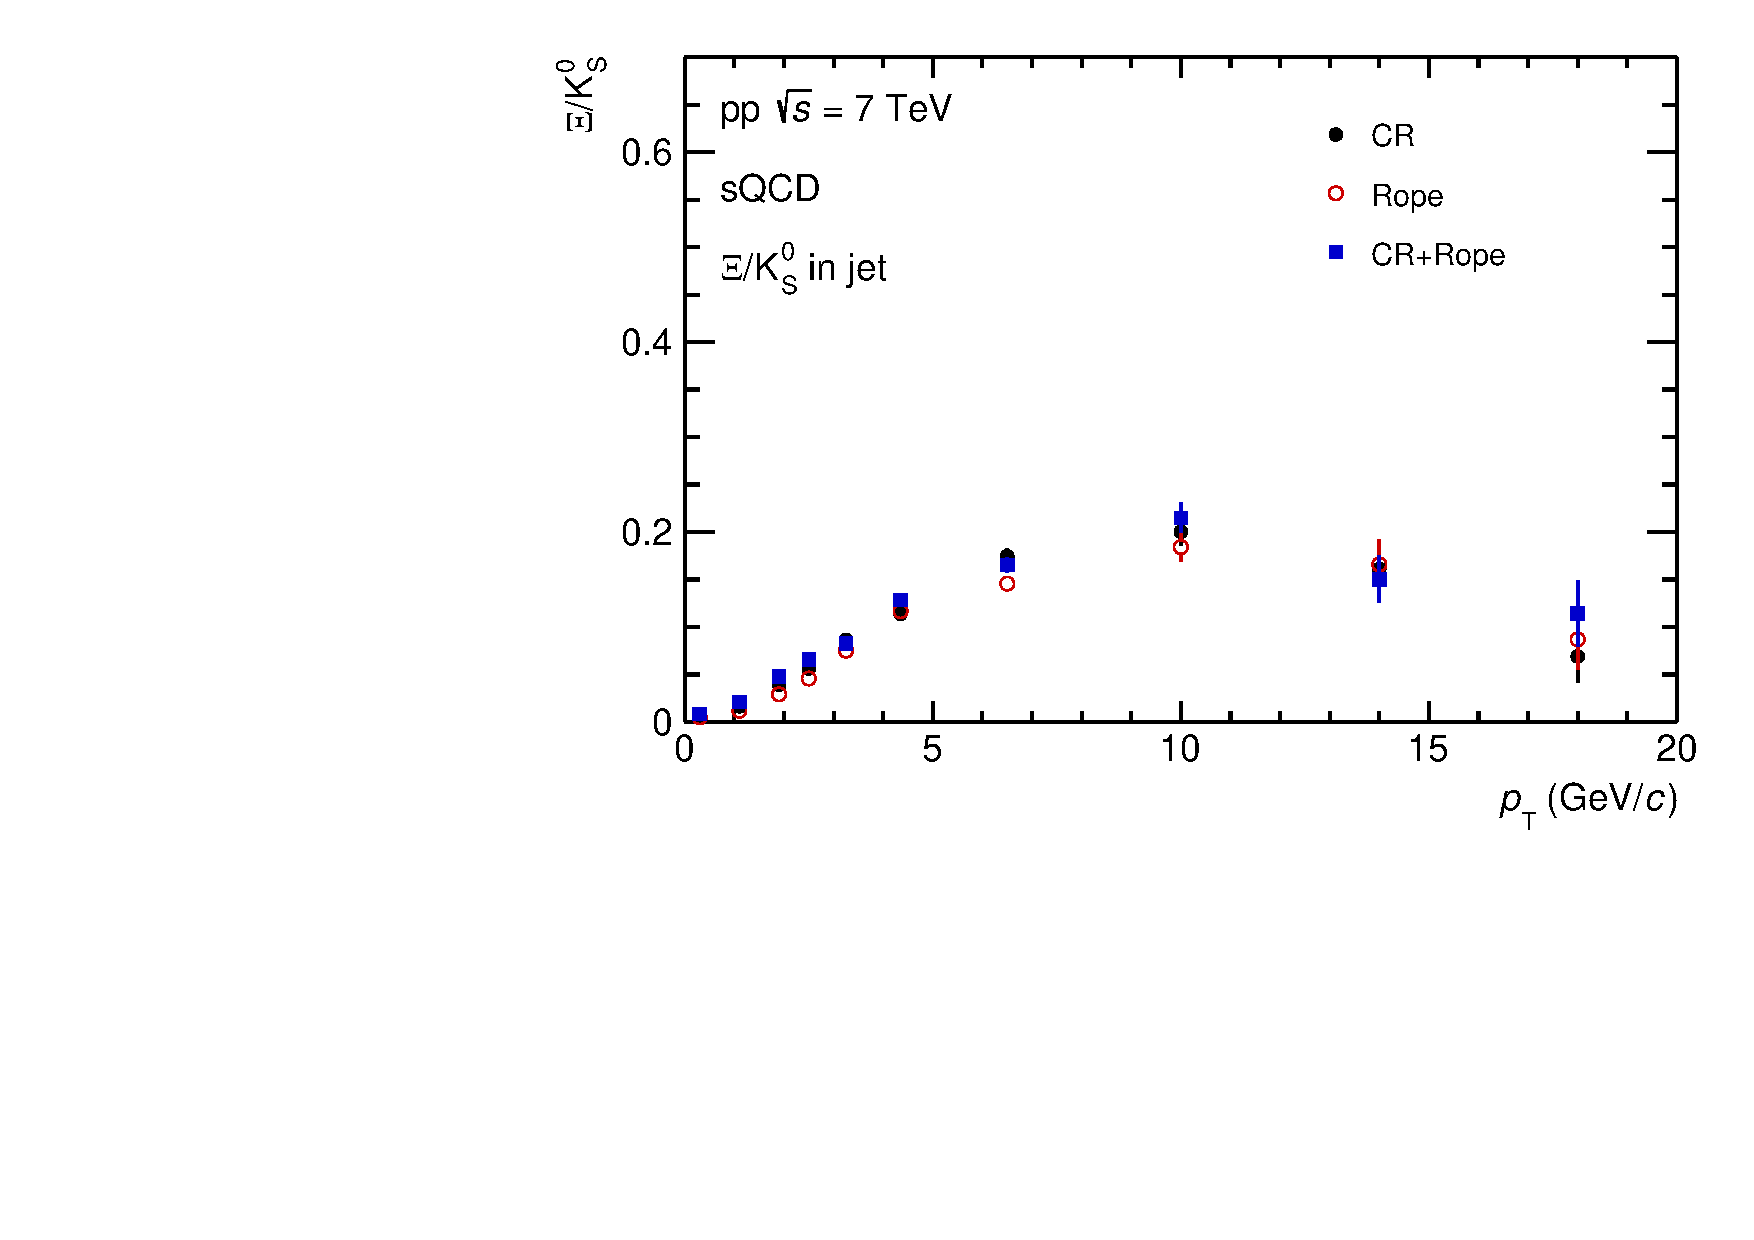
\includegraphics[width=.32\textwidth]{XKRatio_JE}
                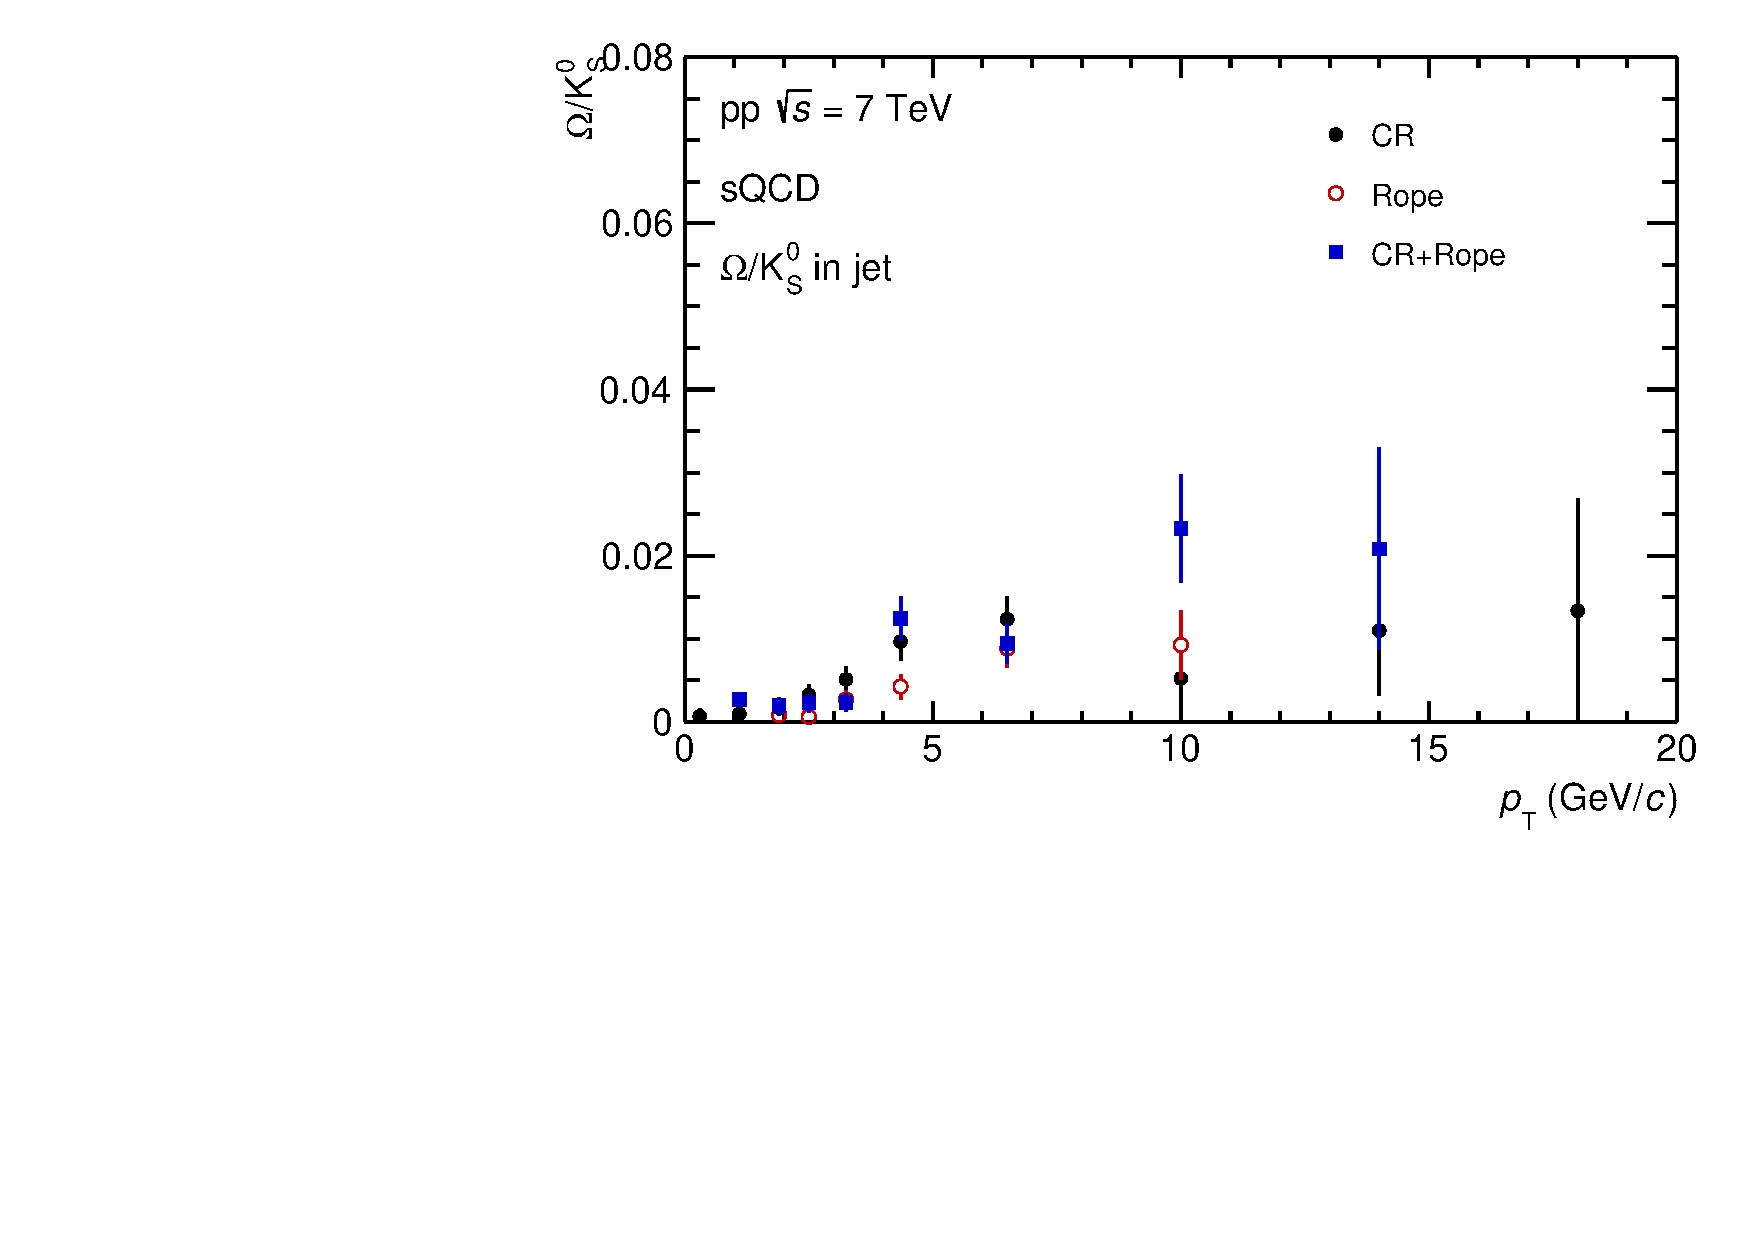
\includegraphics[width=.32\textwidth]{OKRatio_JE}
                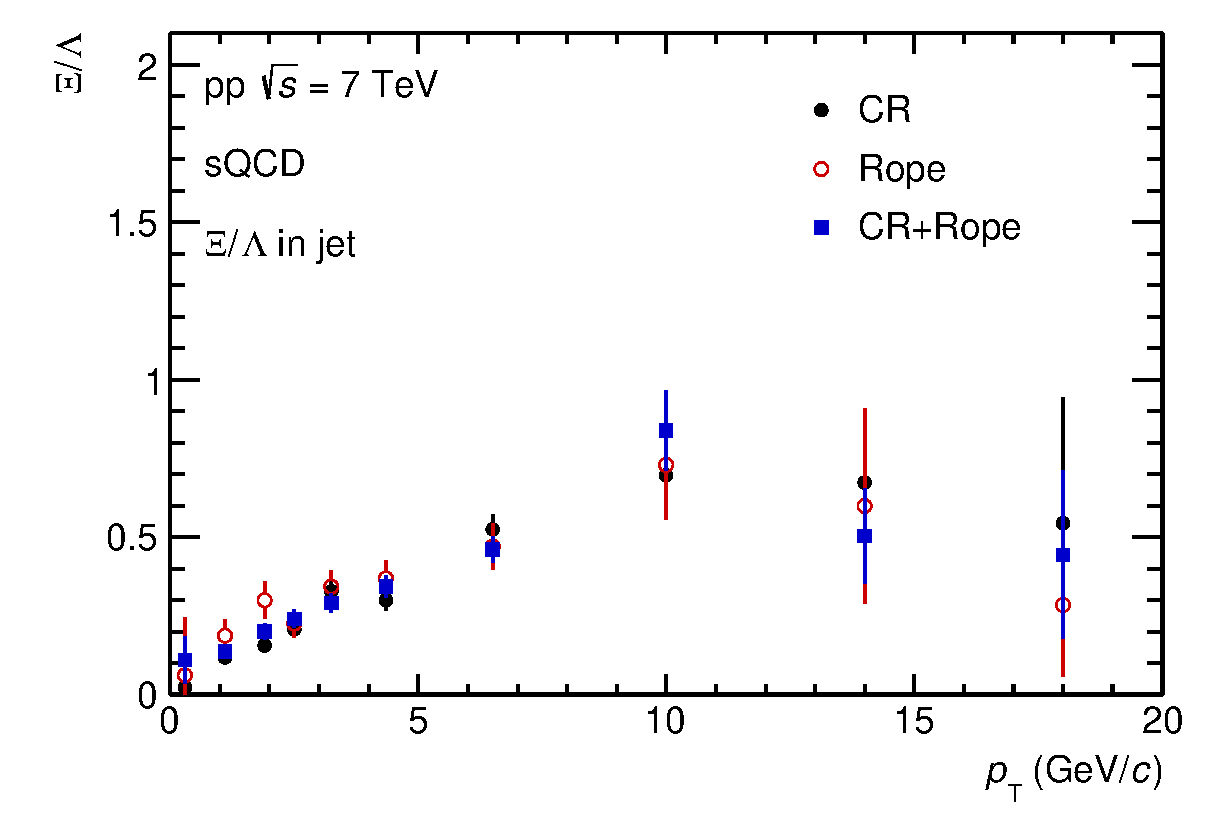
\includegraphics[width=.32\textwidth]{XLRatio_JE}
                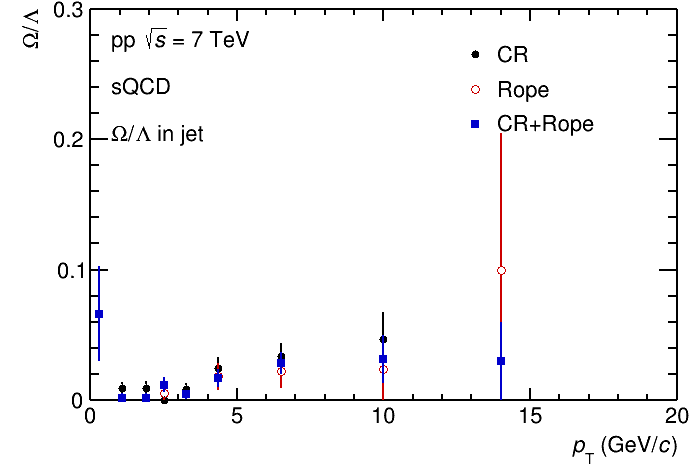
\includegraphics[width=.32\textwidth]{OLRatio_JE}
                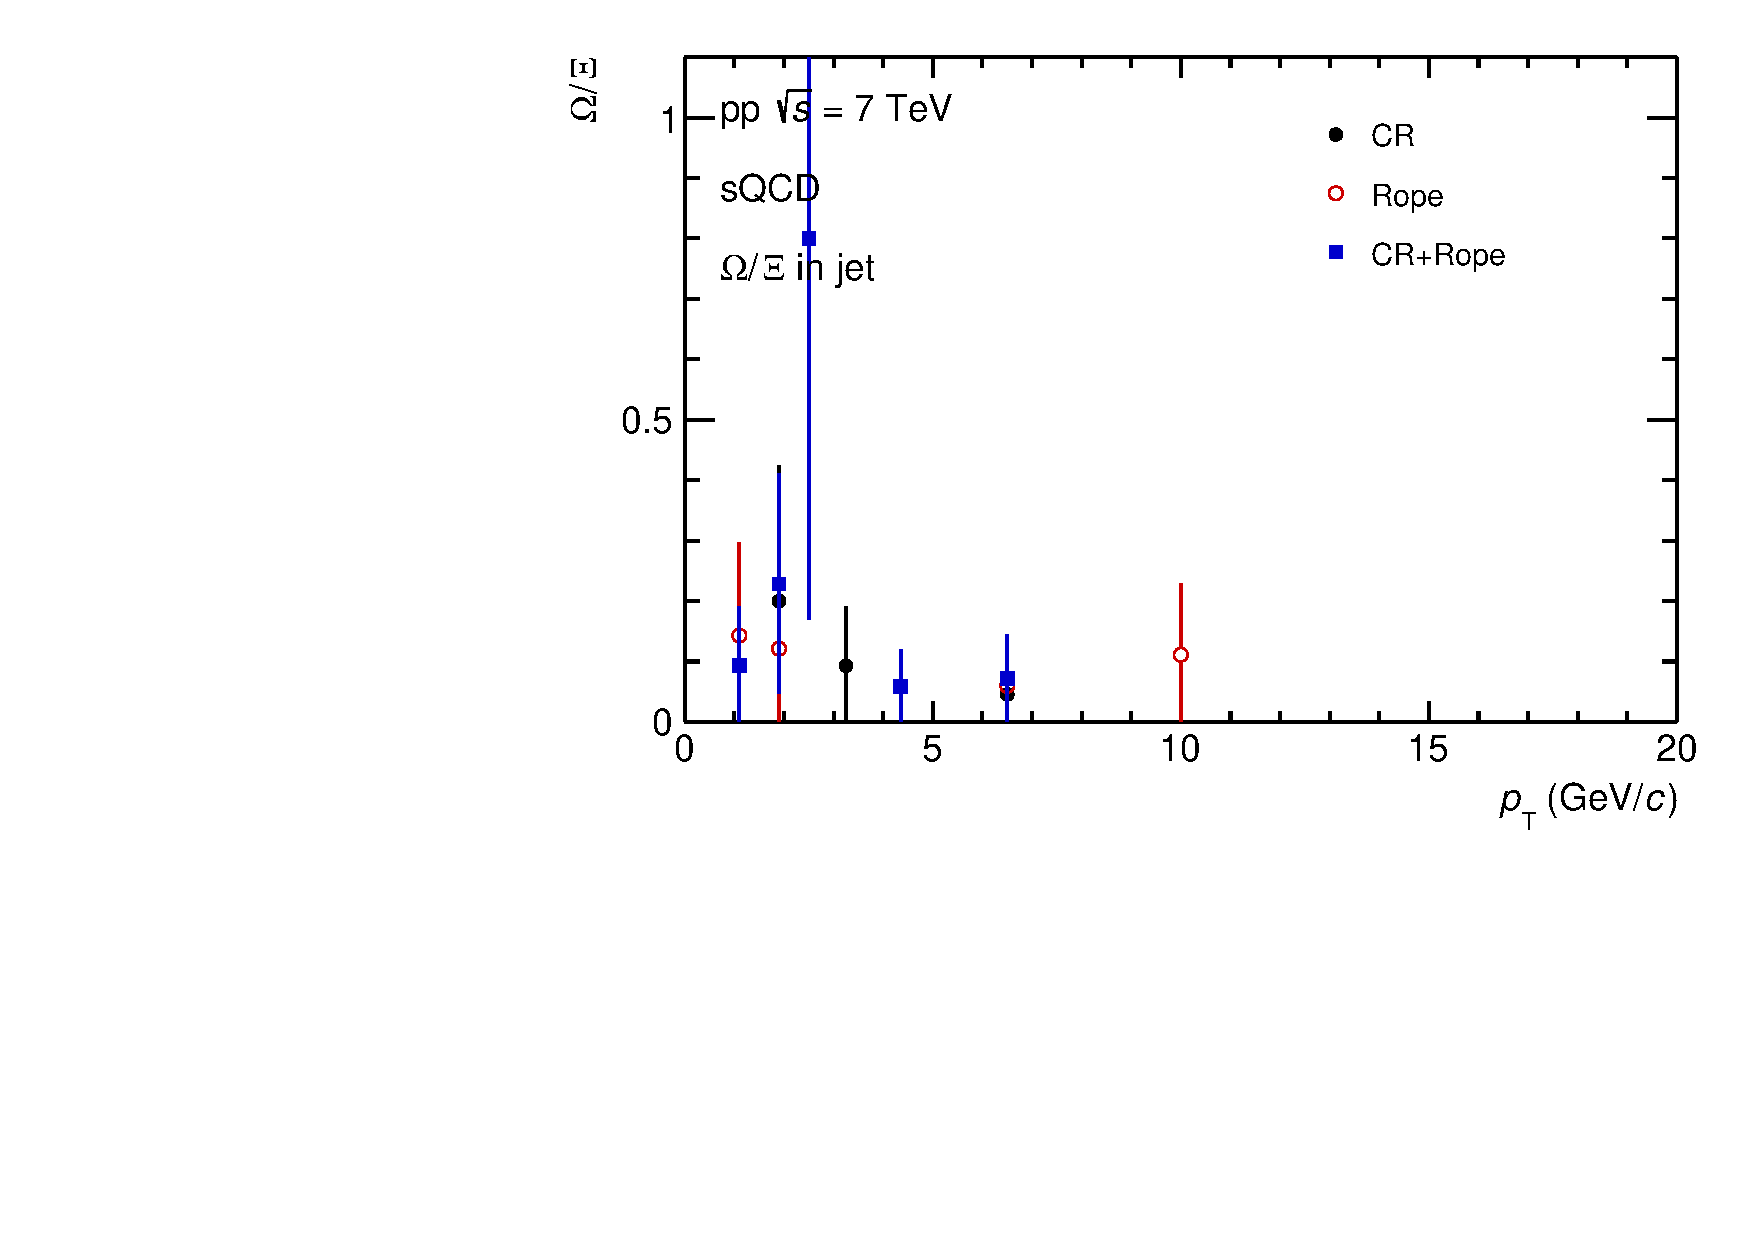
\includegraphics[width=.32\textwidth]{OXRatio_JE}
        \end{center}
        \caption{Baryon-to-meson ratio(top) and Baryon-to-meson ratio(bottom) in jets with $\pT$ distribution.}
        \label{fig:JEParRatio}
\end{figure}

\begin{figure}[ht]
        \begin{center}
                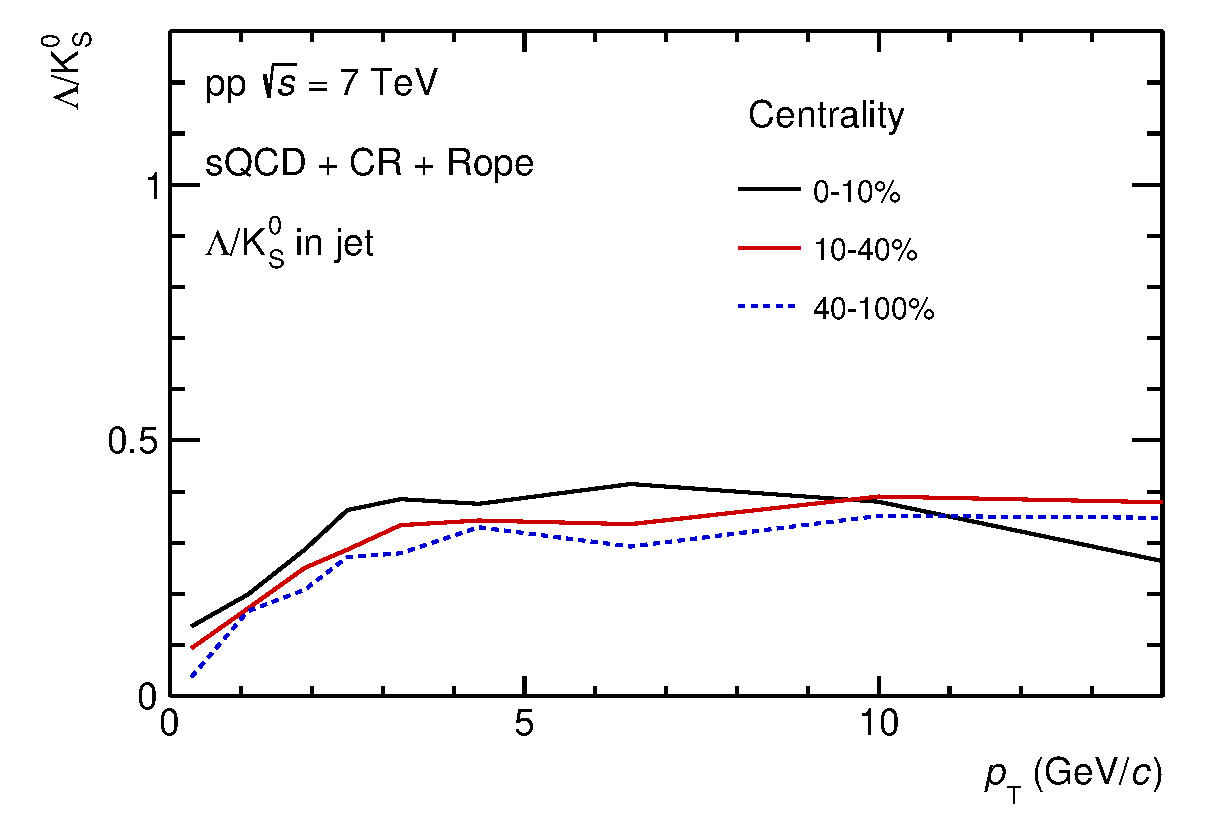
\includegraphics[width=.48\textwidth]{LKRatio_JE_Cent_cr_rope.eps}
                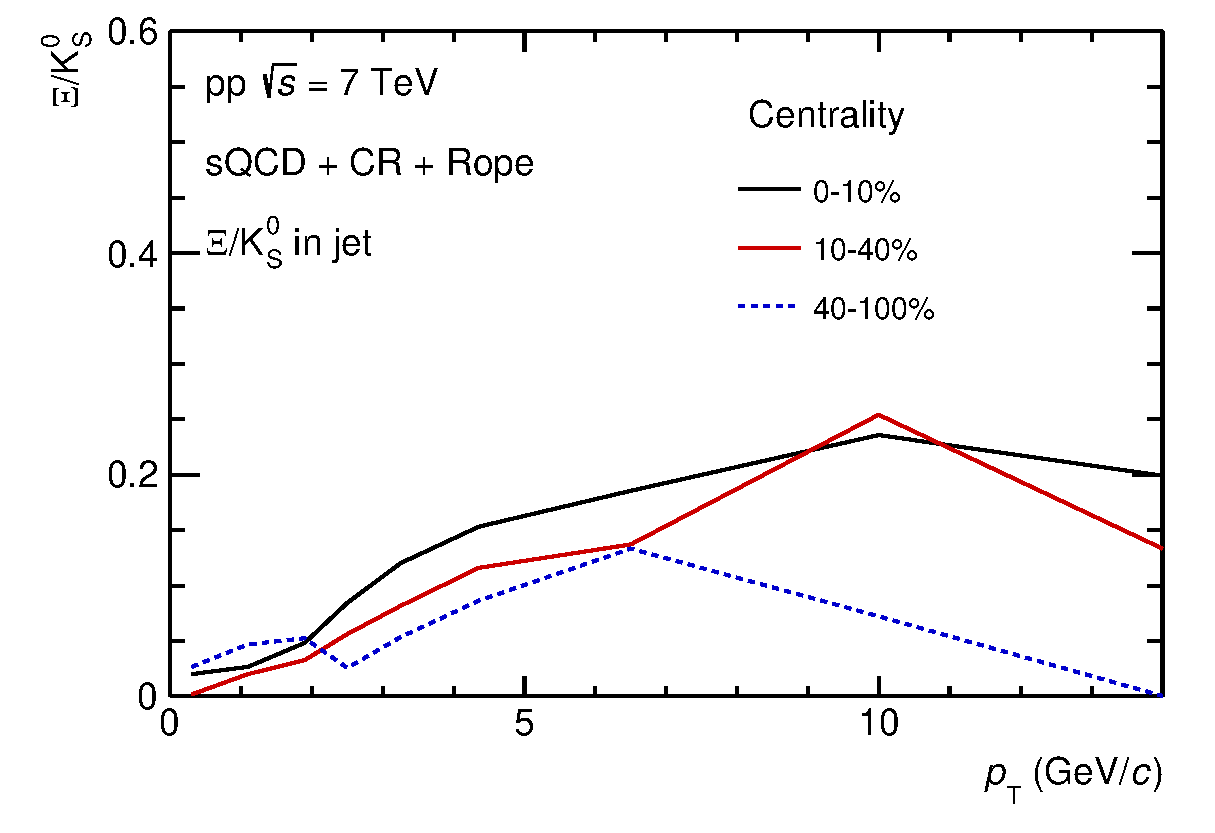
\includegraphics[width=.48\textwidth]{XKRatio_JE_Cent_cr_rope.eps}
                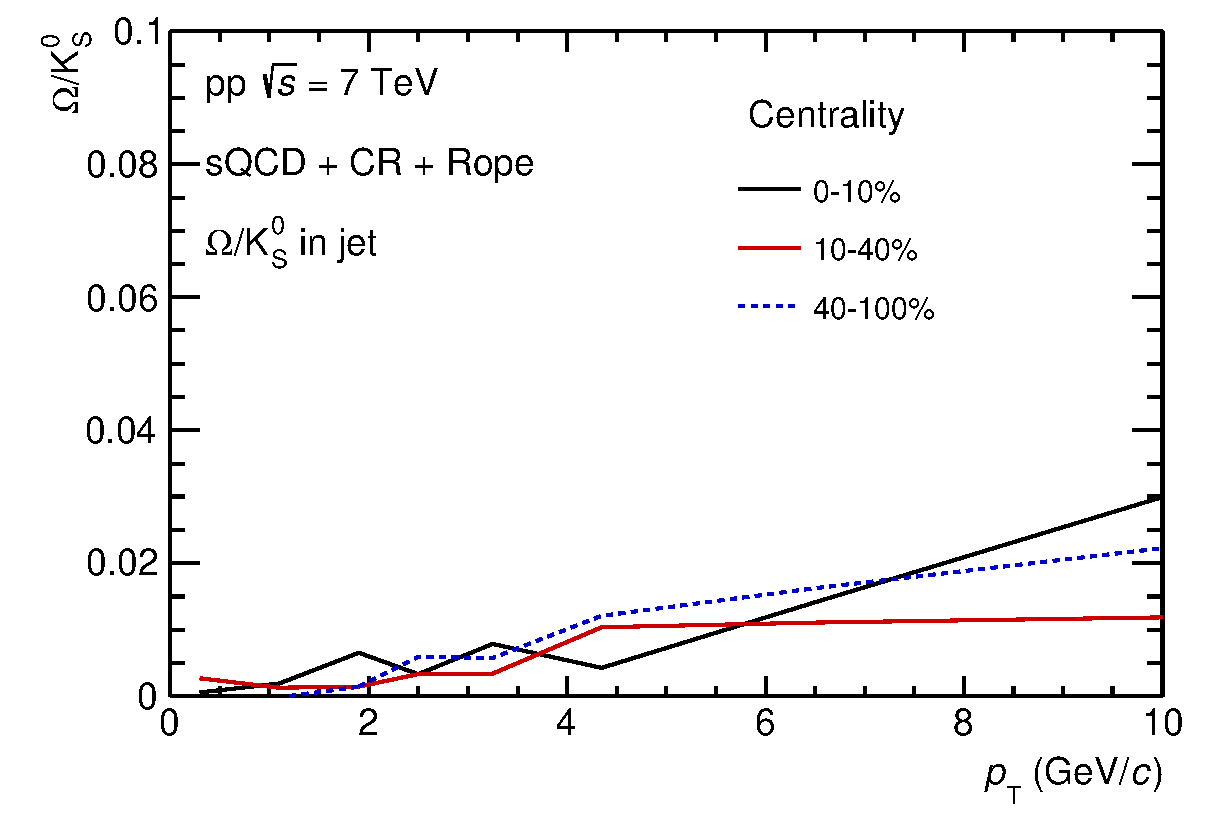
\includegraphics[width=.48\textwidth]{OKRatio_JE_Cent_cr_rope.eps}
                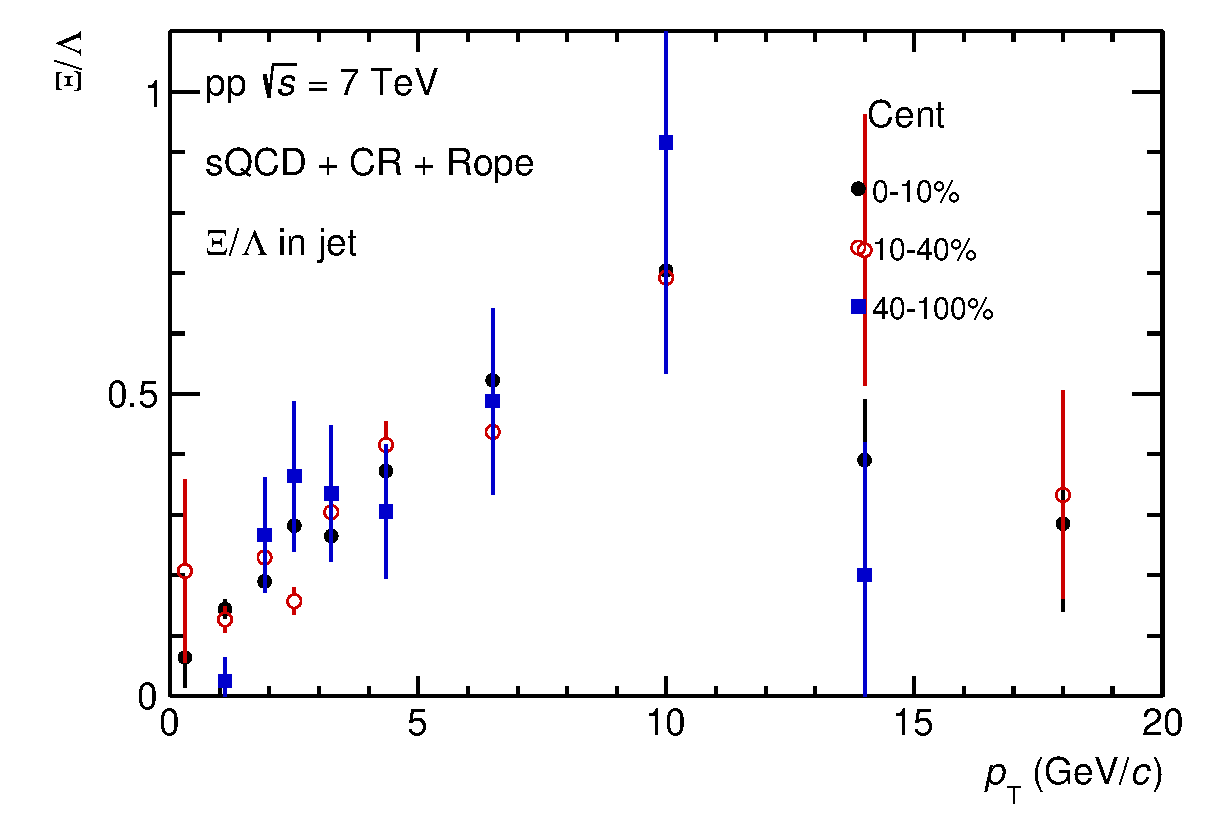
\includegraphics[width=.48\textwidth]{XLRatio_JE_Cent_cr_rope.eps}
        \end{center}
        \caption{Baryon-to-meson ratio(top) and Baryon-to-meson ratio(bottom) in jets with $\pT$ distribution in different centrality bins.}
        \label{fig:JEParRatioCent}
\end{figure}
